\chapter{Estrutura}

\par Baseado nos requisitos estruturais apresentados no PC01 e atualizados na tabela \ref{tab:Requisitos de Estrutura}, a solução de estrutura e abastecimento foi desenvolvida.

\begin{table}[H]
\centering
\begin{tabular}{ | m{2cm} | m{12cm}| } 
 \hline
 \textbf{Requisito} & \begin{center}\textbf{Descrição}
   
 \end{center} \\ 
 \hline
 RFEST01 & Ser de uso intuitivo para o usuário.\\
 & \\
\hline
 RFEST02 & Estruturas físicas compactas e portáteis que deem suporte aos componentes internos e externos a estação. \\
 \hline
 RFEST03 & O material deve ser leve e resistente, capaz de proteger os componentes de eventuais impactos e intempéries provenientes do ambiente e de seu deslocamento. \\
  \hline
RFEST04 & Ter uma estrutura para o usuário e uma outra voltada para o armazenamento do sistema de abastecimento. \\
\hline
RFEST05 & Ter um sistema de transmissão de torque do atuador(motor) para as válvulas-esferas do abastecimento. \\
\hline
RFEST06 & Não gerar interferência no sistema eletrônico.  \\
\hline
RFEST07 & Estrutura interna montável e desmontável, além de ser de fácil manutenção. \\
\hline
RFEST08 & Sistema de abastecimento baseado nos componentes definidos pelo cliente. \\
\hline
\end{tabular}
\caption{Requisitos de Estrutura}
\label{tab:Requisitos de Estrutura}
\end{table}

\begin{figure}[!h]
	\centering
	\label{bateria_maleta}
		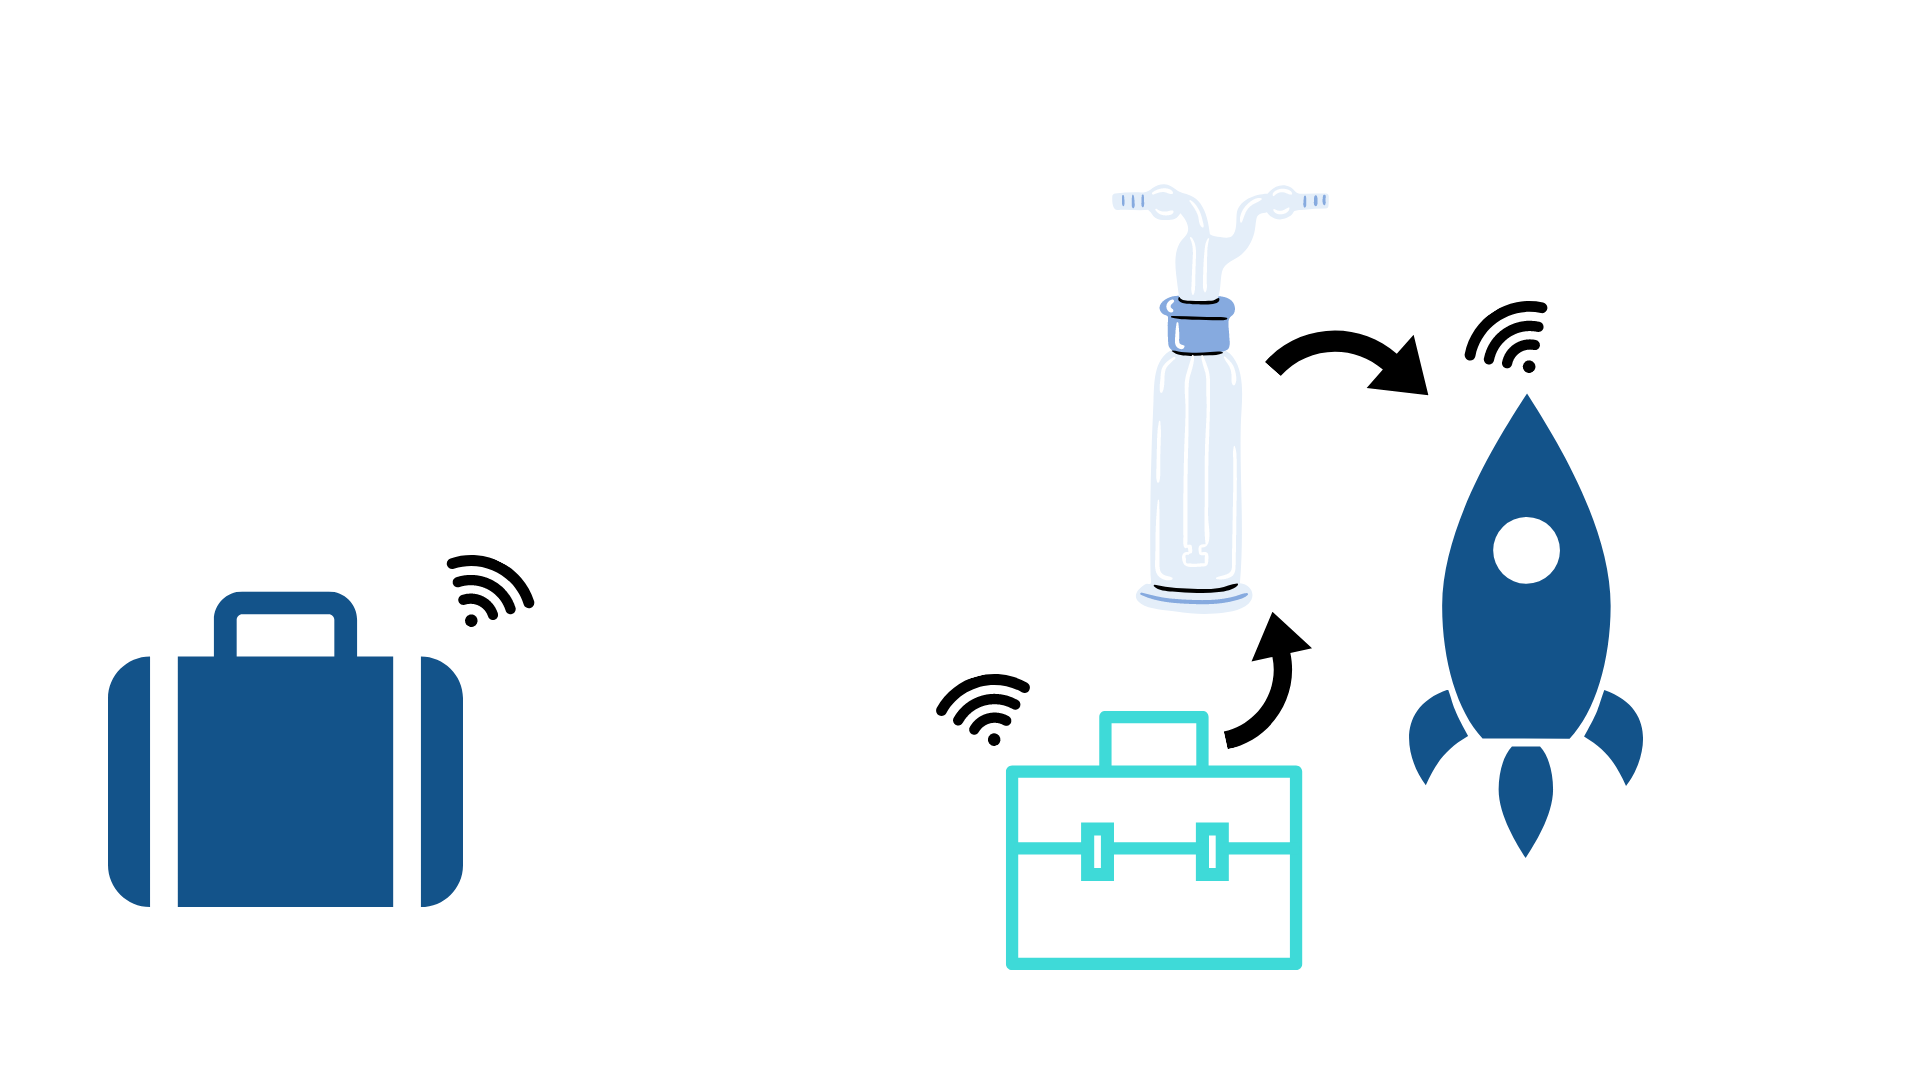
\includegraphics[width=1\textwidth]{figuras/solucao_estrutura.png}
	\caption{Solução estrutural e de abastecimento}
	\label{fig:soluçao_estrut}
	\end{figure}

\par O RGS necessita que todo o produto seja portátil e suficiente para configurar e apoiar as missões de foguetes da CTR. Assim, durante sua concepção estrutural, o principal foco da equipe foi a mobilidade e a robustez para adequação às condições ambientais encontradas nos potenciais locais de lançamento e teste de foguetes. Por isso nossa solução estrutural deve ser equipada com todos os instrumentos necessários para o suporte eletrônico e de software responsáveis por rastrear e comandar o foguete durante o lançamento.

\par Dessa forma, nossa solução se divide em três frentes principais. A primeira é a maleta de usuário, onde ficarão os componentes eletrônicos e a interface de usuário de software (\ref{maleta_01}). Depois tem-se a maleta de suporte, responsável por abrigar os componentes para o abastecimento e a ignição do foguete à distância (\ref{maleta_02}). E, por fim, no próximo capítulo (\ref{abastecimento}) é apresentado a descrição do sistema de abastecimento, com seus componentes em uso integrados até a entrada do foguete. Na figura \ref{fig:soluçao_estrut} pode-se ver como o trabalho estrutural e de abastecimento foi abordado.


\section{Mudanças}
\label{sec:mud_est}

\par A solução estrutural inicial era de desenvolver apenas uma estrutura em formato de maleta, visando que ela fosse o bastante para o uso e carregamento de toda a solução. Porém, depois foi visto que a solução proposta demandaria do cliente o uso de um cabo de energia, muito superior aos comerciais, se tornando um empecilho para a usabilidade do produto. Além de que um cabo elétrico de grandes dimensões possui perda ao longo de sua transmissão, assim foi optado por desenvolver uma solução totalmente segura e sem fios para o conjunto de controle e de abastecimento. 

\par Fazendo-se então necessária a construção de uma segunda estrutura para comportar e transportar os elementos de abastecimento de modo que esse fique perto da base de lançamento, enquanto a outra estrutura fica em uma distância segura com o usuário.

\par Além disto foi-se percebido a necessidade do desenvolvimento de duas cases, uma para comportar o sistema de carregamento das baterias, ou seja, uma estrutura em forma de carregador. Enquanto que a outra destinasse para proteger o sistema eletrônico presente na base de lançamento do foguete.

\par As mudanças visuais mais perceptíveis bem como a evolução do projeto ao longo dos PC's pode ser vista na figura \ref{fig:evolucao}

\begin{figure}[H]
	\centering
	\label{bateria_maleta}
		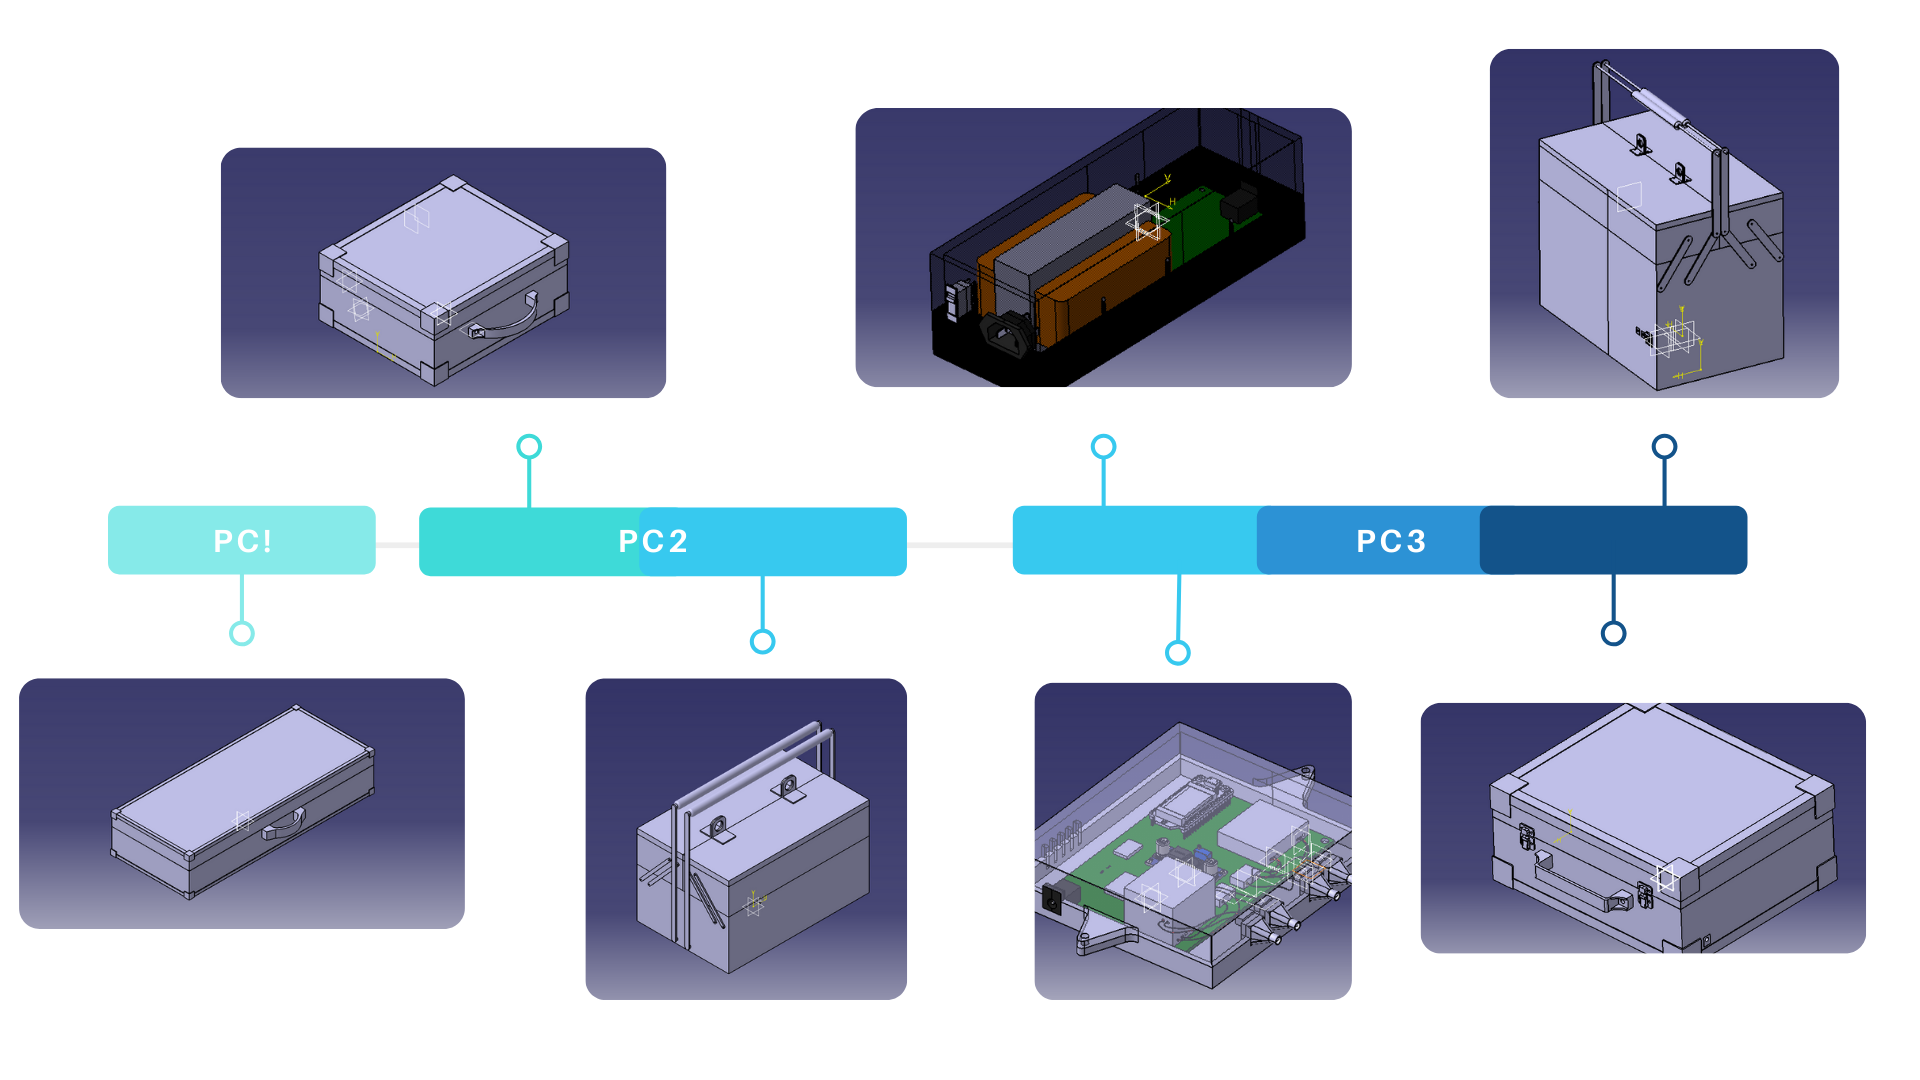
\includegraphics[width=1\textwidth]{figuras/mudanca_estrutura.png}
	\caption{Evolução da solução}
	\label{fig:evolucao}
	\end{figure}

\par Vale-se ressaltar que todas as estruturas aqui apresentadas, foram dimensionadas baseado nos componentes internos que cada uma deverá comportar, bem como para a melhor distribuição e acomodação destes. Além de ter um design condizente com o produto proposto.

\section{Especificações de materiais}
\label{sub:Especificações de materiais}

\par Durante a seleção de materiais, é necessária uma sistematização que permita analisar a vasta possibilidade de combinação de materiais que podem constituir determinado produto a fim de extrair um candidato vencedor, que cumpra com maior eficiência possível os requisitos da aplicação \cite{walterconteudo}.

\subsection{Materiais estruturais}

\par Antes de apresentar a lista em si, é necessário evidenciar as características desejáveis para as estruturas que serão utilizadas na solução. Durante a etapa de escolha do material a ser utilizado, nem sempre é possível contemplar satisfatoriamente todos os aspectos necessários para aquela determinada finalidade. Por isso, tais aspectos são dispostos em ordem de relevância para o projeto, para que a escolha do material seja feita com embasamento teórico dentro da necessidade real do protótipo. 

\begin{enumerate}
    \item O fator mais relevante para a caixa da \textit{ground station} é o correto funcionamento no local de lançamento. A caixa deve estabelecer, por meio de ondas eletromagnéticas, comunicação mútua com o foguete e com o sistema de abastecimento de propelente durante todas as etapas de lançamento. Portanto, o material escolhido \textbf{não deve gerar interferência} nos sistemas de comunicação. 
    \item A usabilidade e a ergonomia vem a seguir, responsáveis por garantir que o usuário consiga ler, de forma clara e precisa, todos os parâmetros relevantes para a missão e que o auxiliará na tomada de decisão. Assim, \textbf{o material utilizado deve ser moldável} para que embarque os componentes necessários e os disponha de maneira adequada, respeitando as suas diferentes geometrias.
    \item O \textbf{custo} é o terceiro fator mais relevante, uma vez que a viabilidade de fabricação do protótipo está diretamente relacionada com seu valor final. Além do material ser acessível do ponto de vista financeiro, é desejável que ele permita agilidade em sua construção, dado que um material difícil de ser trabalhado pode gerar mais horas de trabalho, o que resulta no aumento do valor total da mão-de-obra e, por consequência, aumento do valor final do protótipo.
    \item Como quarta prioridade, a caixa deve ser resistente de maneira que eventuais quedas ou impactos com outros objetos não venha a interferir o seu correto funcionamento. Materiais com boa \textbf{resistência mecânica} podem contemplar tal característica.
    \item Por fim, a portabilidade se faz necessária devida à utilização da caixa ocorrer em lugares de acesso restrito. Logo, a caixa deve ser \textbf{leve e compacta} para facilitar o seu transporte.
\end{enumerate}

\par Além dos aspectos levantados para a construção das maletas, um outro ponto ainda deve ser abordado nesse estudo dos materiais, que é a seleção do material para as cases de eletrônica e de energia. Essas tem como prioridades principais, os mesmos pontos abordados para as maletas porém com mudanças na ordem de prioridade, onde: a) não deve gerar interferência; b) o material utilizado deve ser moldável; c) leve e compacta; d)resistência mecânica; e) custo.

\par Visto os aspectos desejáveis, é apresentado a seguir o estudo de possíveis materiais a serem utilizados no protótipo, bem como a escolha final de uso. Ressaltando-se que dada as mudanças na ordem de prioridades o material a ser selecionado para as maletas irá divergir do material das cases.


\subsubsection{\textit{Medium Density Fiberboard} - MDF}
     \par O MDF é um material fabricado a partir da aglutinação de fibras de madeira com resina sintética – sendo as mais utilizadas à base de ureia formaldeído, tanino formaldeído e melamina ureia formaldeído –  posteriormente submetidas à prensagem em altas temperaturas  \cite{gomes}. Por serem totalmente homogêneos as placas de MDF não apresentam nódulos em seu interior, o que permite que sejam feitos cortes em todas as direções, facilitando a moldagem da peça, além disso por essa sua composição ele permite que as ondas eletromagnéticas possam fluir através dela. 
     
     \par É um material, leve, resistente, fácil de manusear e transportar mas que requer alguns cuidados, como colocar muito peso sobre ele (para isso deve-se considerar a espessura da placa), arrastar objetos sobre ele e o contato com a água, pois apesar de serem resistentes a umidade, não toleram o contato direto com a água. \cite{mdf_site01}
     
    \par Sua superfície é plana e lisa, oferece alta usinabilidade para encaixar, entalhar, cortar, parafusar, perfurar e moldurar, além de reduzir o uso de tintas, vernizes e ótima aceitação de revestimentos \cite{CAMPOS}. Assim por possuir boa trabalhabilidade, o processo de construção pode apresentar satisfatória rapidez. \cite{eleoterio2000propriedades}
    
    \par O custo varia de acordo com a espessura da chapa, por isso alguns valores são como o do metro quadrado de uma chapa de 3 mm que é aproximadamente R\$37,00. Porém já uma chapa de 15 mm custa em media R\$63,00 o metro quadrado. \cite{mdf_site02}
    
    \par As características mecânicas específicas do material variam de acordo com o tipo de fibra e resina utilizadas. Em geral, são vantagens do MDF a alta relação entre resistência mecânica e massa específica, homogeneidade e ausência de defeitos como nós e desvios de grão \cite{eleoterio2000propriedades}. 
    
    \par De acordo com Silva e Gonçalves \cite{da2007avaliaccao}, os MDF são projetados para serem fabricados com densidades entre 0,5 e 0,8 $g/cm^3$. 
    
    \par Na tabela \ref{tab:mdf} é apresentado algumas das principais propriedades físicas e mecânicas de painéis MDF confeccionados com madeira de \textit{Eucalyptus grandis}. \cite{propriedades_mdf}
    
\begin{table}[h]
\centering
\begin{tabular}{|l|l|}
\hline
Densidade              & 0,695 $g/cm^3$ \\ \hline
Módulo de elasticidade & 3776 $MPa$ \\ \hline
Módulo de ruptura      & 36,1 $MPa$ \\ \hline
Resistência a tração   & 1,01 $MPa$ \\ \hline
\end{tabular}
\caption{Propriedades do MDF}
\label{tab:mdf}
\end{table}

\subsubsection{Polímero Reforçado com Fibra de Vidro - PRFV}
    
    \par É um material composto por uma matriz de resina sintética termofixa, como a Resina Epóxi, reforçada com estreitos filamentos flexíveis de vidro, cujo principal constituinte é a sílica \cite{pierin2005estudo}. Dessa forma o PRFV não gera interferência na comunicação com os sistemas. 
    
    \par Possui razoável manuseabilidade, pode ser cortado, perfurado e moldado, porém caso a caixa seja composta por várias peças o encaixe entre elas pode dificultar o processo de montagem.    
    
    \par O processo de fabricação é lento pois é necessária a fabricação do PRFV em si, ou seja, não é vendido o PRFV pronto para uso e sim os filamentos de vidro e a resina. Além disso, o PRFV deve ser confeccionado em um molde que deve ser previamente fabricado com o formato da peça final. O custo de material suficiente para produzir um metro quadrado de PRFV é de R\$53,00.  
    
    \par De acordo com Lin et al (1996), conforme citado por Pierin, os PRFV exibem alta resistência mecânica, porém problemas de deformabilidade e instabilidade, devido à sua baixa elasticidade e rigidez, são os maiores inconvenientes deste material. \cite{pierin2005estudo}
    
    \par De acordo com CALLISTER, a densidade do PRFV varia entre 1,5 $g/cm^3$ podendo chegar até próximo de 3 $g/cm^3$ dependendo dos materiais utilizados. \cite{callister2000ciencia}
    
    \subsubsection{Polímero Reforçado com Fibra de Carbono - PRFC}
    
    \par Similar ao PRFV, o PRFC utiliza como reforço fibras compostas principalmente de carbono que resultam da pirólise de fibras plásticas, como a poliacrilonitrila (PAN). 
    
    \par O processo de fabricação do PRFC é análogo ao processo de fabricação do PRFV. O material para produzir um metro quadrado PRFC custa aproximadamente R\$335,00 \cite{fc_kit}. Enquanto que a folha de fibra de carbono flexível de alta dureza sai a R\$65,00 o metro quadrado. \cite{fc_placa}
    
    \par Segundo Galli as fibras de carbono são normalmente empregadas em aplicações que requerem elevadas propriedades mecânicas (alta resistência mecânica e alto módulo de elasticidade) associadas a uma baixa densidade. \cite{galli2016caracterizaccao}
    
    \par Na tabela \ref{tab:PRFC} é apresentado algumas das principais propriedades físicas e mecânicas do PRFC. \cite{HOLOS5320} e \cite{vanicomparaccao}
    
    \begin{table}[h]
\centering
\begin{tabular}{|l|l|}
\hline
Densidade              & 1,78 $g/cm^3$ \\ \hline
Módulo de elasticidade & 380 $MPa$ \\ \hline
Módulo de ruptura      & 124,5 $MPa$ \\ \hline
Resistência a tração   & 102,9 $MPa$ \\ \hline
\end{tabular}
\caption{Propriedades do PRFC}
\label{tab:PRFC}
\end{table}
    
\subsubsection{Poli Ácido Lático - PLA}
    
    \par O PLA é um polímero termoplástico feito através da extração do milho, trigo ou cana de açúcar passando por várias etapas de produção. Sua composição permite o correto funcionamento dos sistemas de comunicação. 
    
	\par O PLA é um material comumente usado em prototipagem rápida onde uma impressora 3D deposita o material partindo de dados provenientes de sistemas de desenho assistido por computador (CAD). Sua alta fluidez e baixa contração durante o processo de extrusão permite a produção de peças com alta precisão dimensional e bom acabamento superficial.
	
	\par O filamento de PLA para impressão 3D tem valor médio de R\$120,00 o kg com a possibilidade e facilidade de poder encontrá-los em diversas cores \cite{pla}. O valor de processamento do PLA para projetos com baixas unidades é muito elevado, tornando inviável seu processamento por injeção ou \textit{vacuum forming} e impressão 3D.  
	
	\par De acordo com Simões, o PLA é um material rígido e resistente, difícil de deformar ou flexionar, possui alta dureza, que o torna com baixa resistência ao impacto. É um material indicado para produção de protótipos que não sejam submetidos às condições de altos esforços mecânicos, atritos ou altas temperaturas.c\cite{simoes2009mechanical}
	
	\par Na tabela \ref{tab:PLA} é apresentado algumas das principais propriedades físicas e mecânicas do PLA. \cite{santana2018comparative}

    \begin{table}[h]
\centering
\begin{tabular}{|l|l|}
\hline
Densidade              & 1,24 $g/cm^3$ \\ \hline
Módulo de elasticidade & 2690 $MPa$ \\ \hline
Módulo de ruptura      & 53,32 $MPa$ \\ \hline
Resistência a tração   & 50,0 $MPa$ \\ \hline
\end{tabular}
\caption{Propriedades do PLA}
\label{tab:PLA}
\end{table}

\subsubsection{Acrilonitrila Butadieno Estireno - ABS}
    
    \par Para  Vossen,  o  ABS é  um  termoplástico  que  consiste em uma  fase  de  borracha  (butadieno)  dispersa  em  uma  matriz de  SAN  (copolímero  de  acrilonitrila  Estireno),  também denominado terpolímero. \cite{vossen2009nanocompositos}
    
	\par A acrilonitrila confere estabilidade ao calor e resistência química e à flexão; o butadieno é responsável pela resistência ao impacto e tenacidade; já o estireno por sua vez é responsável pelo brilho, rigidez e fácil processamento. Devido à suas propriedade e baixo custo o ABS se tornou um material bastante utilizado por várias indústrias. O ABS pode ser Processado por injeção, extrusão e sopro.
	
	\par O valor do ABS depende da forma em que você o deseja, o kg do ABS granulado custa em média R\$ 16,80 já o kg do filamento de ABS para impressão custa em media R\$80,00. O valor de processamento do ABS para projetos com baixas unidades é muito elevado, tornando inviável seu processamento por injeção ou \textit{vacuum forming} e impressão 3D. \cite{abs01}
	
	\par Assim as propriedades do ABS dependem do teor de cada componente, mas em geral o ABS apresenta boa resistência térmica e ao impacto, alta estabilidade dimensional, alta rigidez, alta dureza, baixa absorção de umidade, etc. \cite{junior2014aspectos}
	
	\par Na tabela \ref{tab:ABS} é apresentado algumas das principais propriedades físicas e mecânicas do PLA. \cite{abs}

    \begin{table}[h]
\centering
\begin{tabular}{|l|l|}
\hline
Densidade              & 1,05 $g/cm^3$ \\ \hline
Módulo de elasticidade & 1335,9 $MPa$ \\ \hline
Módulo de ruptura      & 29,0 $MPa$ \\ \hline
Resistência a tração   & 62,0 $MPa$ \\ \hline
\end{tabular}
\caption{Propriedades do ABS}
\label{tab:ABS}
\end{table}

\subsubsection{Resultado}

\par A partir dos dados apresentados para os diferentes materiais, é possível chegar às seguintes conclusões: os materiais selecionados para o estudo são caracterizados por não gerarem interferência, aspecto imprescindível para o projeto. 

\par Assim, o próximo aspecto a ser analisado é o usinabilidade e geometrias que o material pode assumir com poucos processos. Nesse quesito, os materiais com fibras se tornam menos atraentes por sua complexa usinabilidade. Já no quesito custo os materiais mais comerciais possuem melhor custo benefício como é o caso do MDF e dos filamentos de impressão. 

\par Porém, as características mecânicas e físicas são o fator decisivo para a escolha do material, com a menor densidade entre os materiais selecionados e o maior módulo de elasticidade, o MDF, se saiu na frente nos dois últimos critérios analisados. Apesar da sua baixa resistência a tração, o fato de o sistema desenvolvido não estar sujeito a esse tipo de carga faz com que ele se torne ainda mais atrativo. Logo, o material escolhido para a confecção dos protótipos das maletas foi o \textbf{MDF 15mm}.

\par Walter sinaliza que a dinâmica de Seleção de Materiais e Processos de Fabricação devem ser flexíveis a ponto de permitir sua utilização em etapas desde o \textit{Design} Conceitual ao Projeto para Manufatura \cite{walterconteudo}. 

\par Tratando-se de um projeto de engenharia, foi definida a escolha de mais de um material para a construção das estruturas principais, já que suas partes possuem funções diferentes. Assim a carcaça da caixa será feita em com um material de revestimento, apresentado  na seção \ref{revestimento}, o que permite um acabamento melhorado e uma proteção em caso de eventual contato com líquidos, uma fraqueza vista no MDF anteriormente. 

\par Os componentes estruturais serão feitos em MDF de madeira de eucalipto, visto que a mesma segue o enquadramento para construção de painéis de uso estrutural determinado pela especificação NBR 15316-2 \cite{propriedades_mdf}. Assim combinando diferentes materiais, tem-se uma diminuição dos custos de produção, diminuição do peso e aumento das propriedades mecânicas se comparado aos polímeros.

\par Para as cases, visto que elas precisam ser mais compactas as opções 3D são mais atrativas, por causa da espessura e da sua usinabilidade acessível. Entre as opções apresentadas o com propriedades mecânicas mais condizentes com o projeto é o PLA. Por isso o material escolhido para as cases foi o \textbf{PLA}. 

\subsection{Material para revestimento da caixa}
\label{revestimento}

\par Para aumentar a resistência do material que forma as estruturas da estação de controle, recomenda-se o seu revestimento com material polimérico (i.e. borracha), de modo a aumentar sua resistência à abrasão, impacto, cortes e pressão. Em aplicações industriais, alguns desses polímeros são desenvolvidos para ser aplicados em condições extremas, a temperaturas muito altas ou em locais com presença de ácidos concentrados, o que foge do escopo do uso no projeto, de proteger a estação de intempéries ambientais e a choques mecânicos moderados, ou seja, queda de uma altura não superior a de uma pessoa carregando a maleta nas mãos: 1 a 1,5 m.

\begin{itemize}
    \item \textbf{Borracha de Etileno Propileno Terpolímero - EPDM }
    \par Material bastante usado para resistência térmica, mas também por sua dureza e por sua impermeabilidade à água. \cite{EPM}
    \item \textbf{Borracha de Estireno Butadieno - SBR} 
    \par Boa resistência à abrasão e resistência moderada a agentes atmosféricos (luz solar, oxigênio). Baixa resistência a ácidos fortes, solventes e a altas temperaturas (acima de 85ºC), o que extrapola a usabilidade esperada do material. \cite{SBR}
    \item \textbf{Borracha de Poliisopreno - IR}
    \par Propriedades muito próximas a da borracha natural. Grande resistência a abrasão, rasgo, mas baixa resistência a agentes atmosféricos (luz solar, oxigênio), que afetam seu envelhecimento. \cite{IR}

\begin{table}[h!]
\centering
\begin{tabular}{|l|l|l|l|}
\hline
Propriedade & EPDM & SBR & IR \\ \hline
Dureza Shore A & 40-90 & 30-95 & 15-100 \\ \hline
Tensão de Rotura (MPa) & 7-18 & 7-21 & 15-25 \\ \hline
Resistência elétrica (ohms/cm$^2$) & 2 x 10$^{16}$ & 10$^{15}$ & 10$^{15}$ \\ \hline
Limites de temperatura (ºC) & -55 a 130  & -45 a 85 & -50 a 80 \\ \hline
Preço (R\$/m$^2$) & \href{https://produto.mercadolivre.com.br/MLB-695763984-manta-lona-epdm-para-lagos-preco-por-metro-quadrado-_JM#position=1&amp;type=item&amp;tracking_id=6d0c4fc5-9267-481f-bd5d-3235e740025b}{140,00}  & \href{https://produto.mercadolivre.com.br/MLB-1582301221-lencol-de-borracha-manta-30mm-x-1mt-largura-_JM#position=1&amp;amp;type=item&amp;amp;tracking_id=496d45a3-ab4a-4895-879d-bae69aa0cf97}{80,00}  & \href{https://produto.mercadolivre.com.br/MLB-1515451183-lencol-piso-manta-borracha-liso-preto-2mm-x-1000mm-_JM#position=2&amp;type=item&amp;tracking_id=06606e66-abe1-4c02-8649-c7365eef54cb}{100,00}  \\ \hline
\end{tabular}
\caption{Propriedades material de revestimento}
\label{tab:revestimento}
\end{table}

\end{itemize}

\par A partir dos dados apresentados na tabela \ref{tab:revestimento} é possível ver que o material para revestimento com o melhor custo beneficio é o \textbf{SBR}, assim esse se torna o material escolhido para o revestimento. 

\section{Maleta 01 - GCS}
\label{maleta_01}

\par A maleta GCS é responsável por enviar o sinal de lançamento do foguete e colher os dados de telemetria deste. Dessa forma, ela tem que armazenar alguns componentes essenciais para que consiga realizar essa função e o usuário consiga analisar e colher os dados obtidos. Para armazenar todos esses componentes, foi pensado em uma maleta com \textit{design} mais robusto, porém, compacta. Suas especificações podem ser verificadas no Apêndice \ref{Drafts_do_projeto}.

\par Como pode ser observado nas figuras \ref{fig:Render Maleta GCS01} e \ref{fig:Render Maleta GCS02}, em sua base ficarão armazenados os componentes eletrônicos e de energia, tais como fontes, baterias e reguladores. Ainda em sua base, para proteger os componentes eletrônicos e o usuário tem-se um fundo falso que serve como meio de acesso aos componente eletrônicos para manutenções e serve também de nicho para o teclado. Já em sua parte superior, a maleta conta com um outro fundo falso que permite acesso à tela de 9" e à base da antena.

\begin{figure}[H]
    \centering
        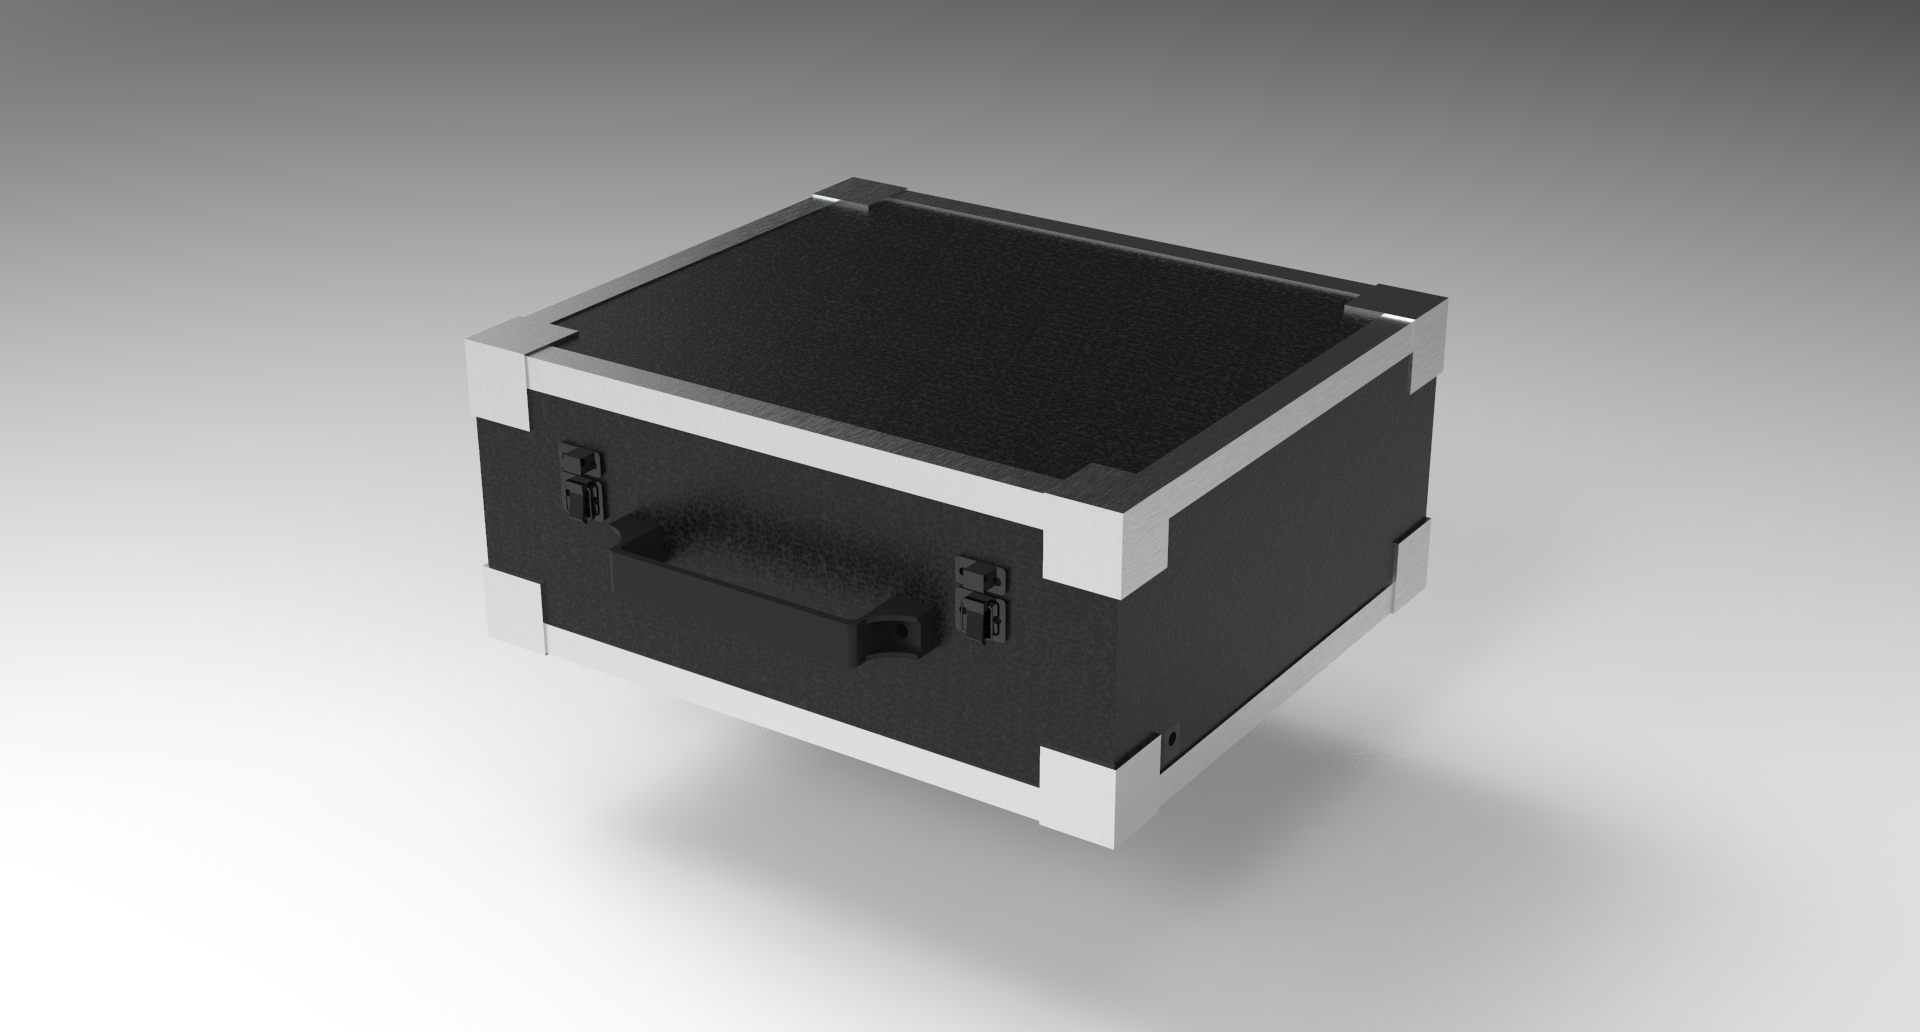
\includegraphics[width=0.7\linewidth]{figuras/untitled.17.jpg}
    \caption{\label{fig:Render Maleta GCS01} Maleta 01 - GCS Fechada}
\end{figure}

\begin{figure}[H]
    \centering
        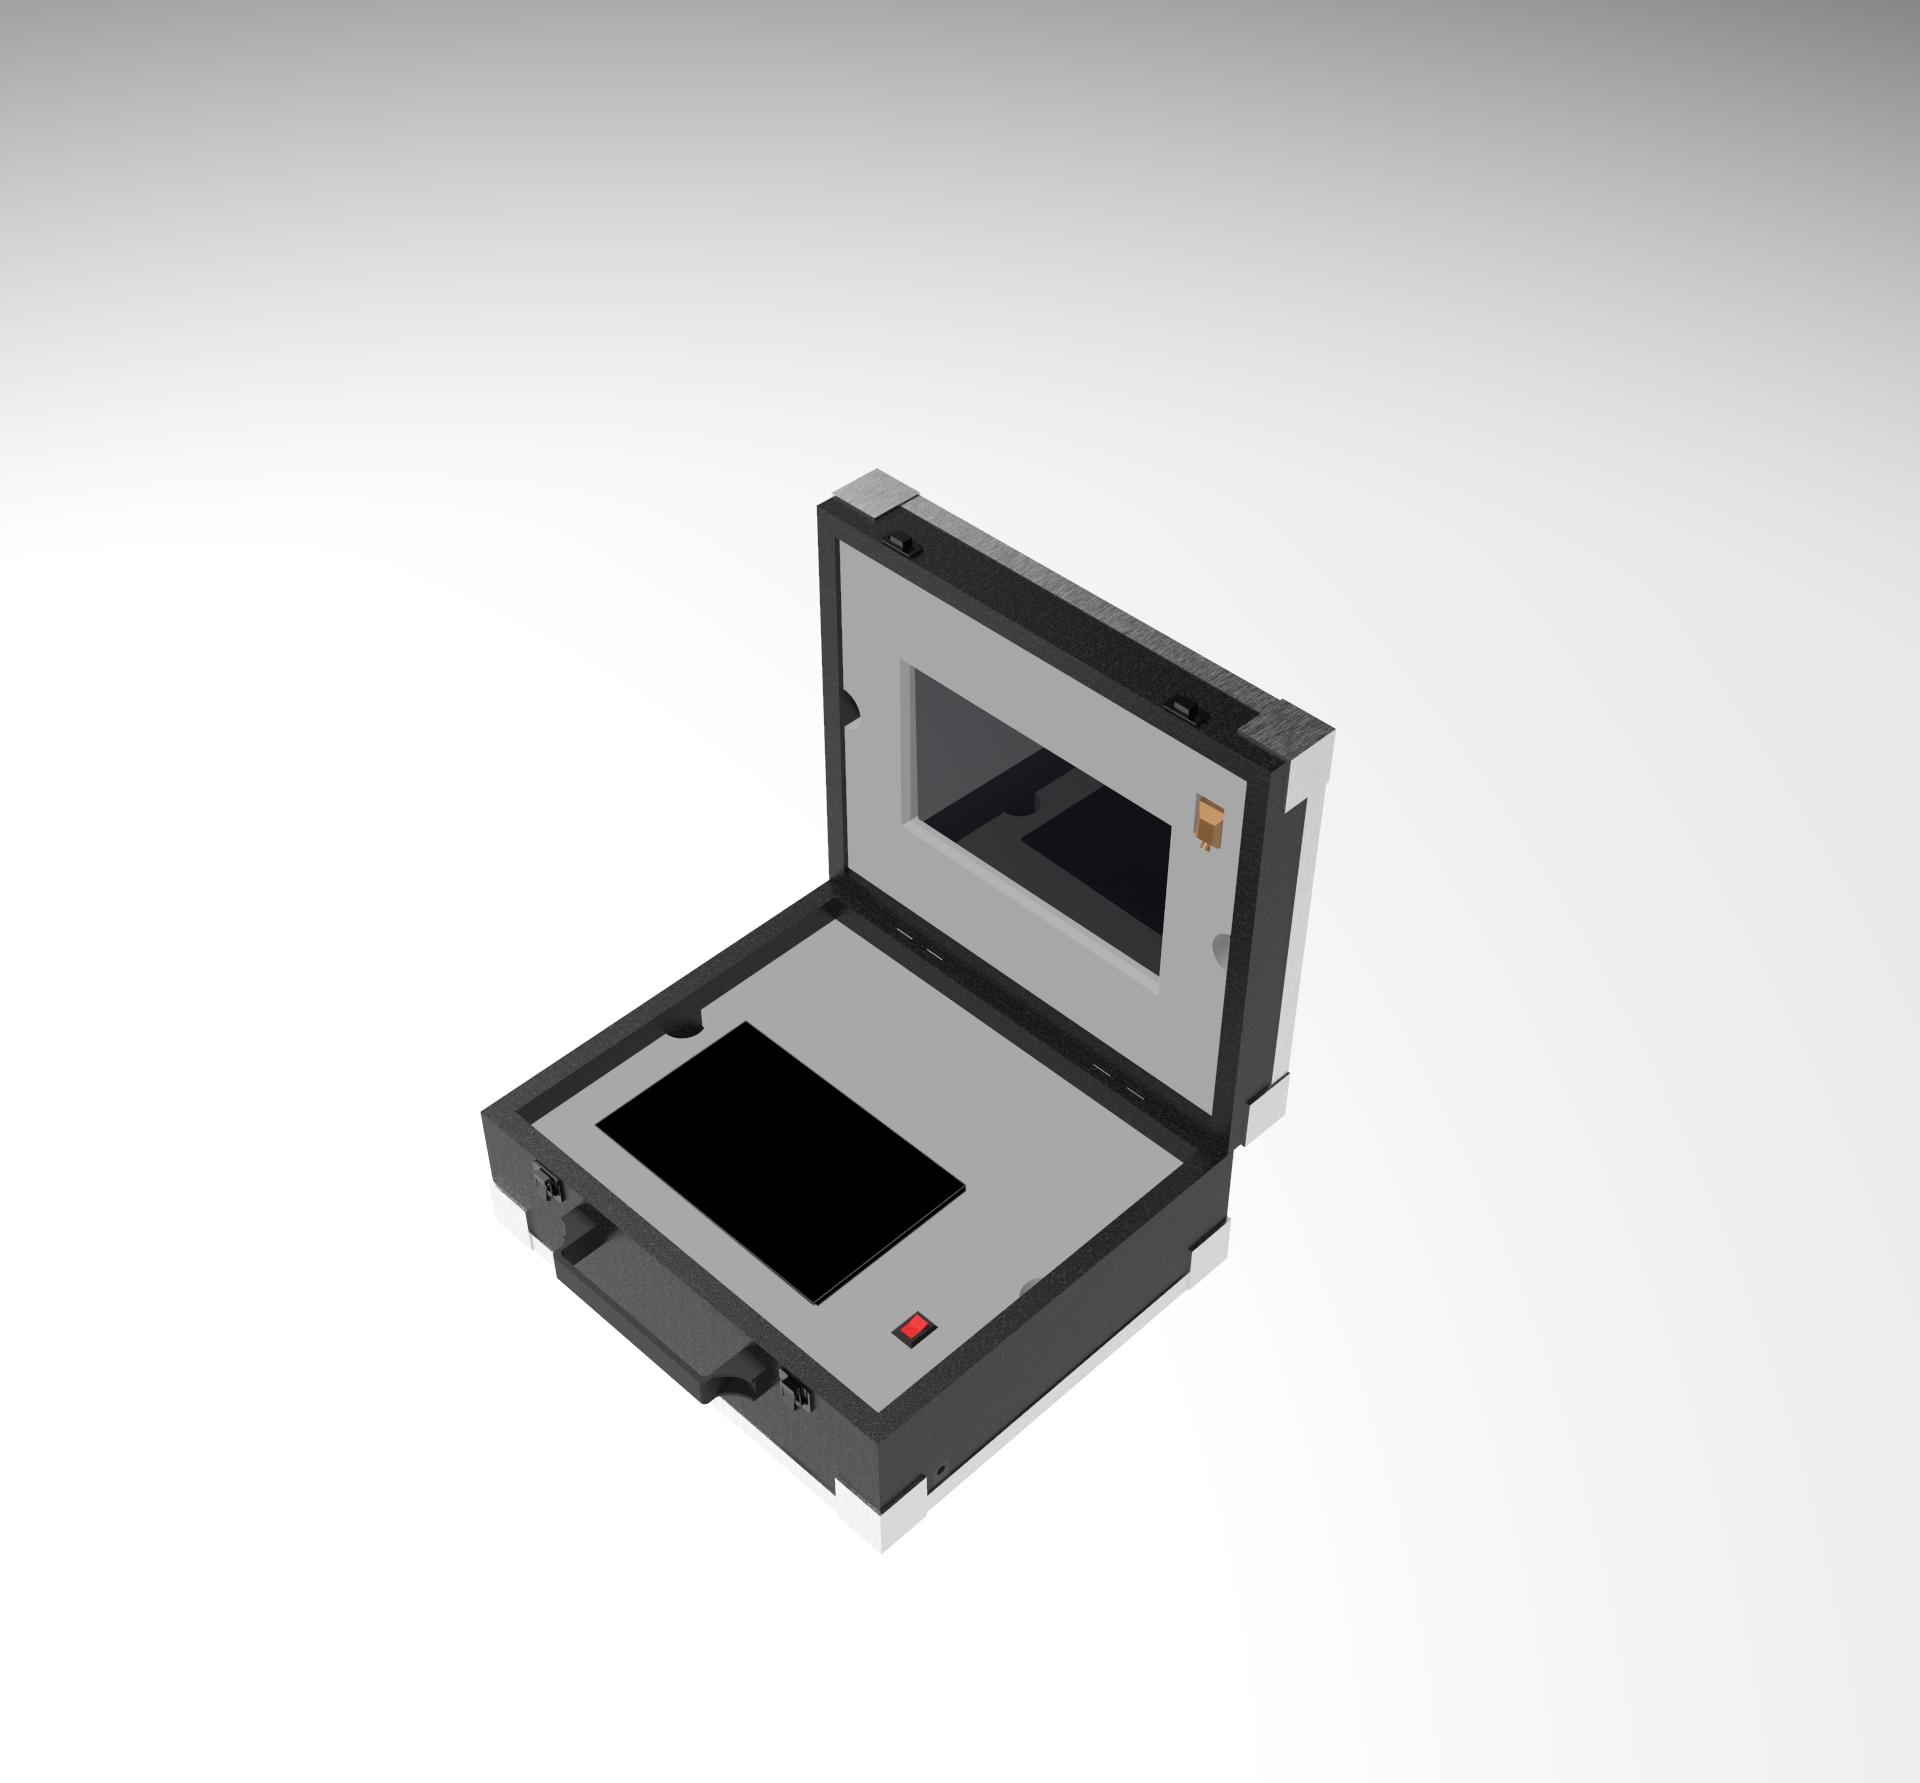
\includegraphics[width=0.7\linewidth]{figuras/untitled.18.jpg}
    \caption{\label{fig:Render Maleta GCS02} Maleta 01 - GCS Aberta}
\end{figure}

\par A disposição dos equipamentos eletrônicos, bem como o interior da base da GCS, podem ser observados na figura \ref{fig:Disposicao dos Componentes}. Já o peso da maleta GCS será de aproximadamente 5 kg, essa estimativa foi realizada utilizando a ferramenta \textit{Measure Inertia} do software CATIA.

\begin{figure}[H]
\centering
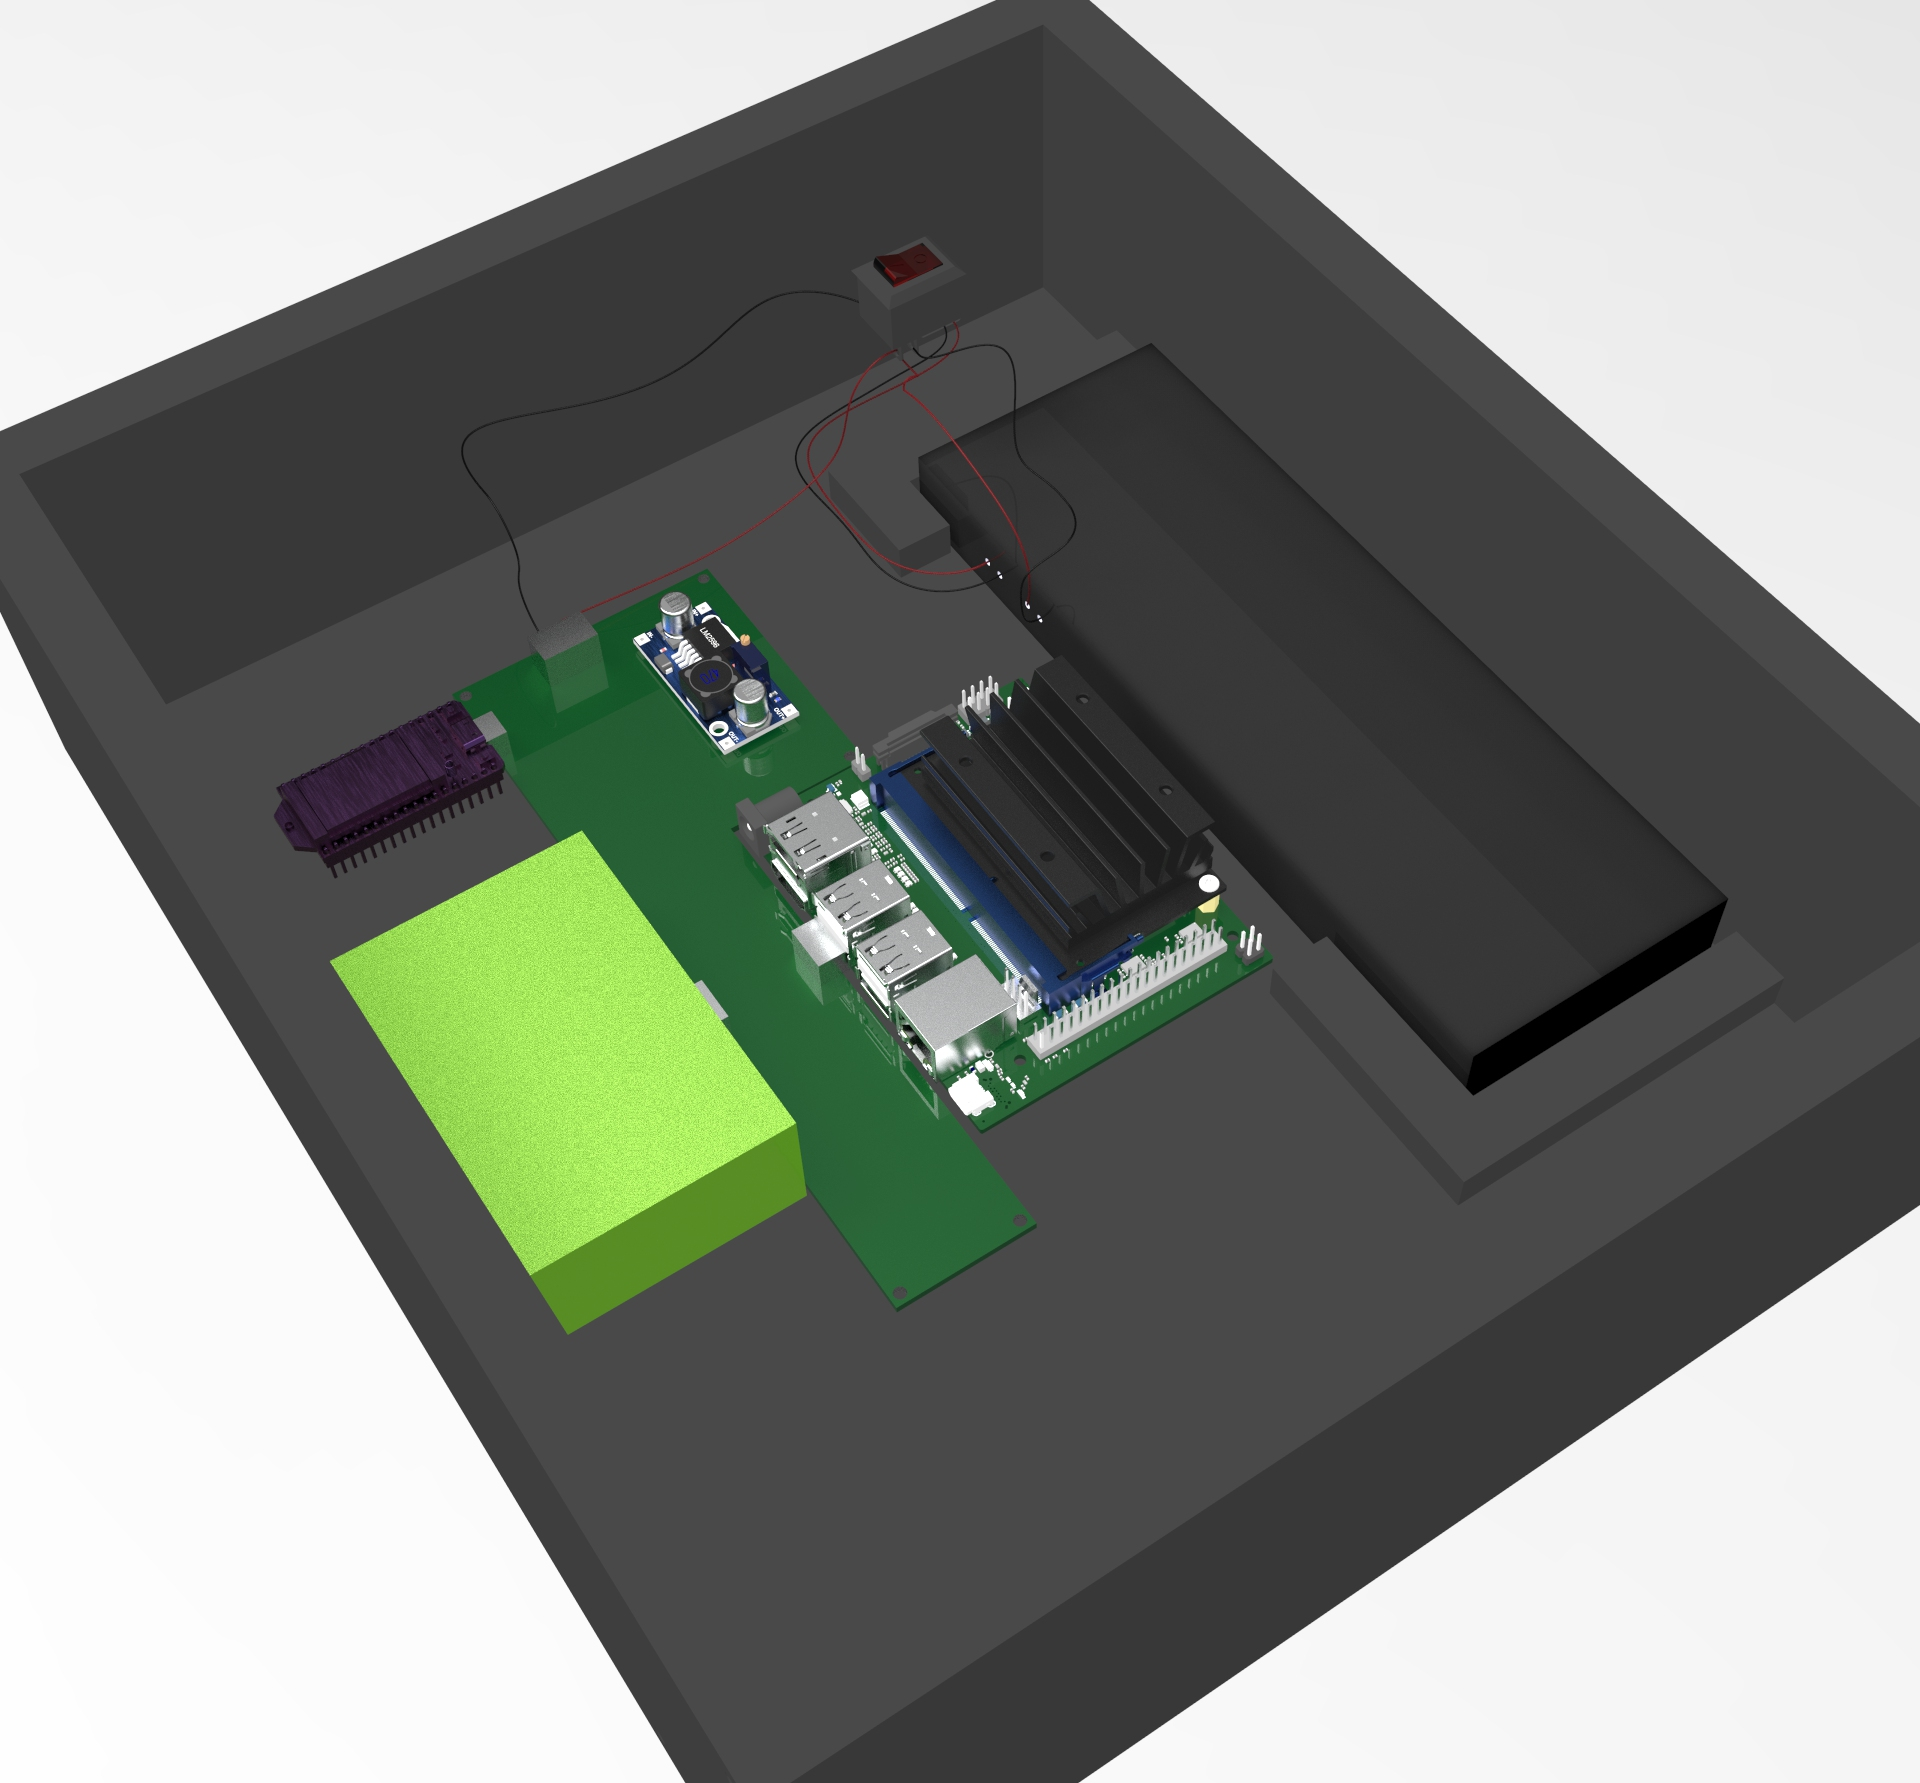
\includegraphics[width=0.5\textwidth]{figuras/untitled.22.jpg}
\caption{Disposição dos equipamentos eletrônicos}
\label{fig:Disposicao dos Componentes}
\end{figure}


\section{Maleta 02 - Abastecimento}
\label{maleta_02}

\par A maleta de abastecimento tem como função transportar os atuadores, as válvulas, a mangueira de abastecimento e a bateria que proporcionará a energia necessária para o acionamento dos mesmos. Dessa forma, a maleta teve seu design inspirado em uma caixa de ferramentas. 

\par A maleta possuirá dois níveis. A base irá acomodar a mangueira e a bateria, fazendo que este seja o espaço com maior área útil na maleta. Já o nível superior é composto por duas áreas de armazenamento simétricas, com o objetivo de acomodar os adaptadores motor-válvula. A distribuição da maleta pode ser observada nas figuras \ref{fig:Render Maleta Alimentacao01} e \ref{fig:Render Maleta Alimentacao02}. É possível observar as especificações para a produção da maleta no Apêndice \ref{Drafts_do_projeto}.

\begin{figure}[H]
\centering
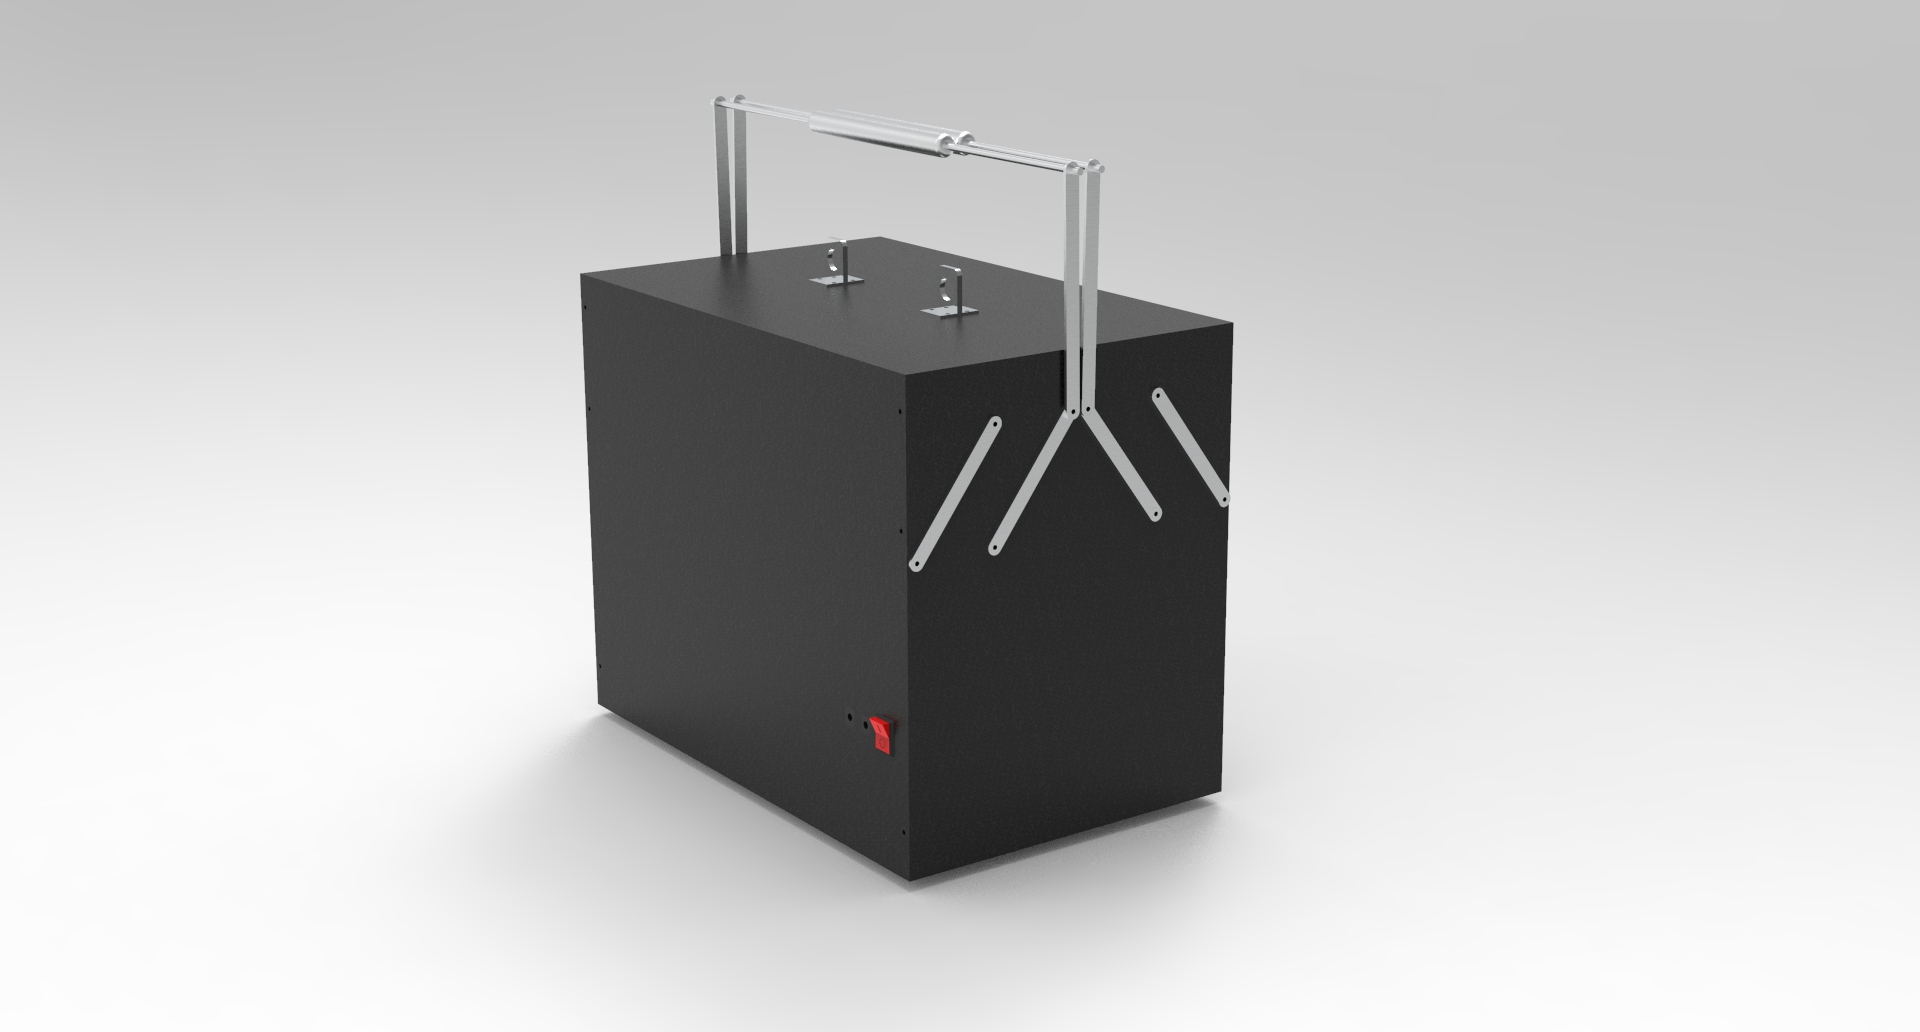
\includegraphics[width=0.7\textwidth]{figuras/cad/untitled.4.jpg}
\caption{Maleta 02 - Abastecimento Fechada}
\label{fig:Render Maleta Alimentacao01}
\end{figure}

\begin{figure}[H]
\centering
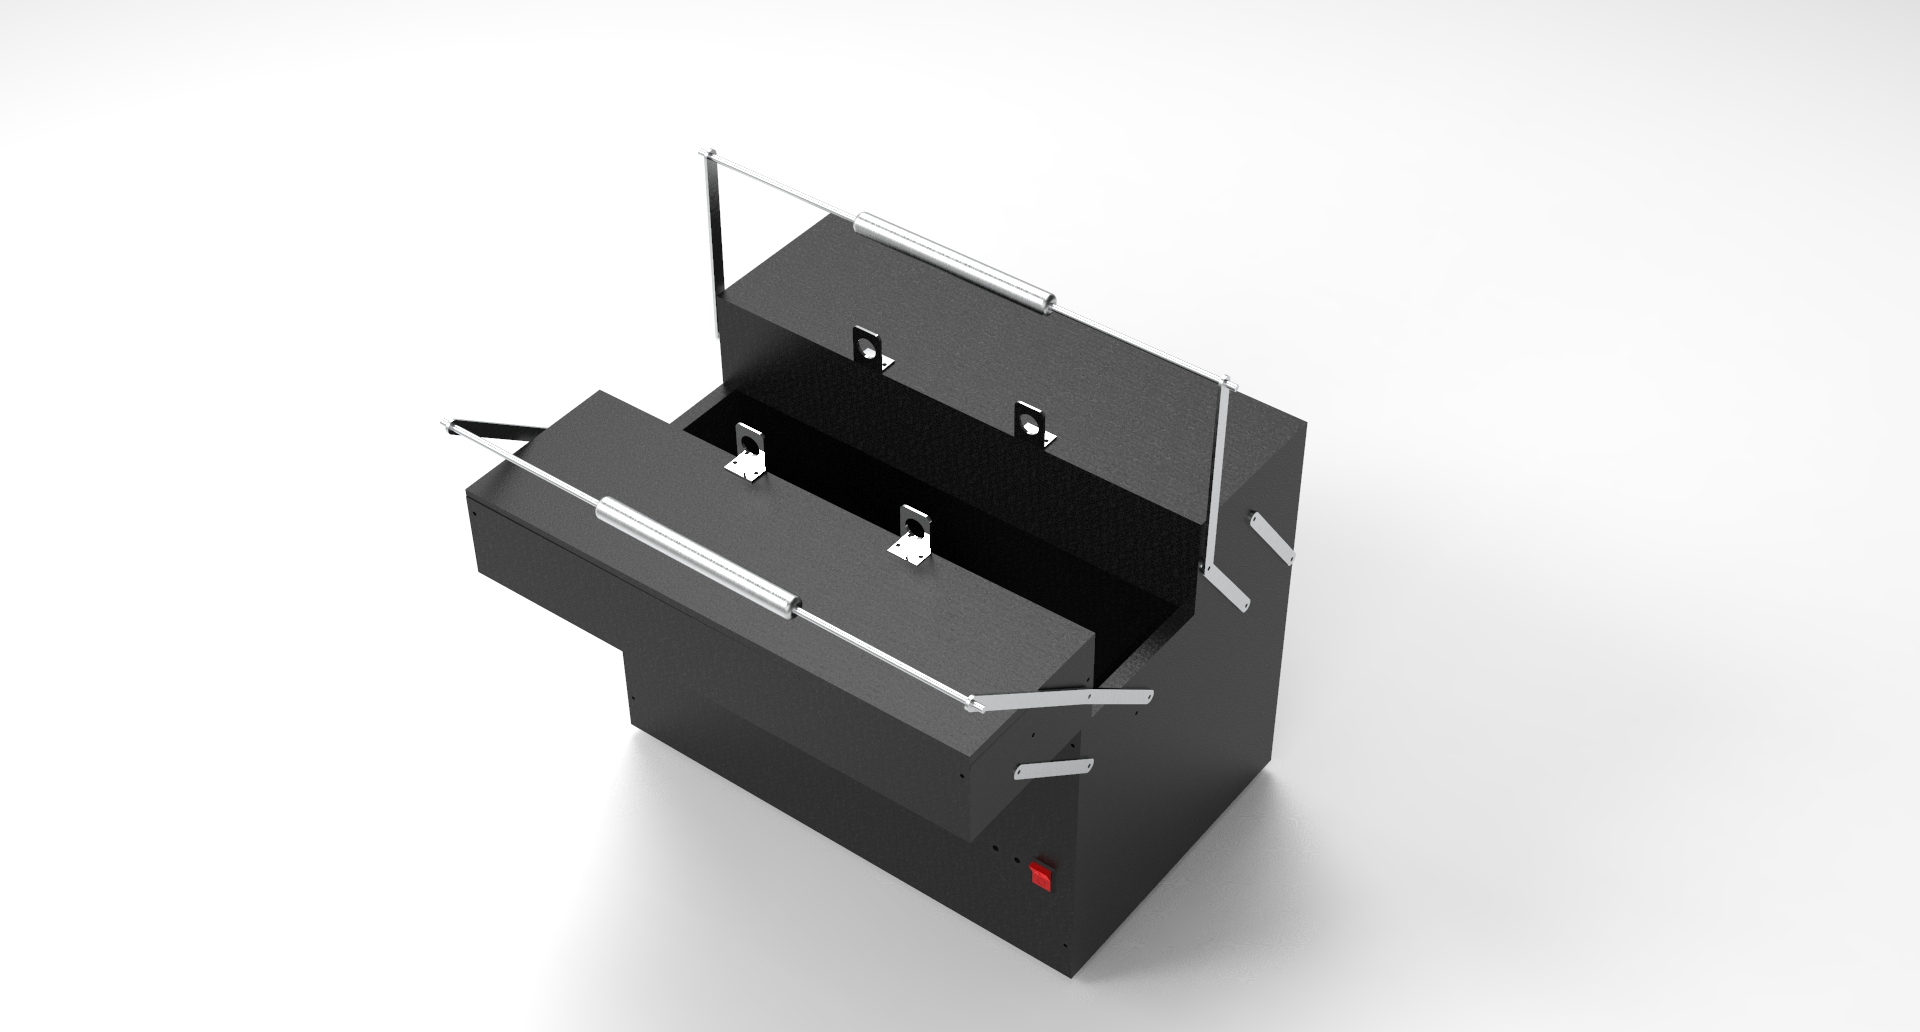
\includegraphics[width=0.7\textwidth]{figuras/cad/untitled.5.jpg}
\caption{Maleta 02 - Abastecimento Aberta}
\label{fig:Render Maleta Alimentacao02}
\end{figure}

\par O peso estimado para a maleta de abastecimento foi de aproximadamente 10 kg. O peso desta maleta foi estimado por meio da ferramenta \textit{Measure Inertia} do software CATIA.

\section{Cases}

\subsection{Carregador}

\par A estrutura do carregador foi desenvolvida para comportar a PCI desenvolvida pelo grupo de energia na seção \ref{sec:carregador}, e os outros componentes pertinentes ao sistema, como condutores e interruptor. 

\begin{figure}[H]
\centering
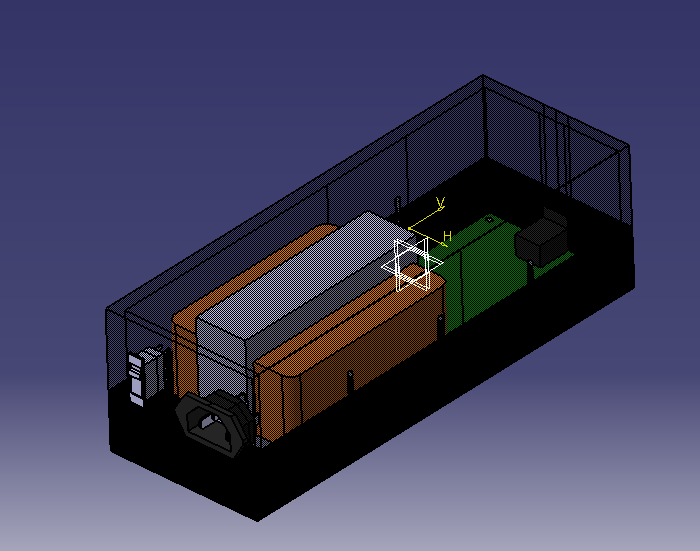
\includegraphics[width=0.7\textwidth]{figuras/cad/ISOCARREGADOR.PNG}
\caption{Vista Isométrica do Carregador}
\label{fig:carregador01}
\end{figure}

\par Na figura \ref{fig:carregador01} é possível vê a vista isométrica do sistema de carregamento, como produto final. Já na figura \ref{fig:carregador02} é visto como fica a distribuição dos componentes dentro da case.  

\begin{figure}[H]
\centering
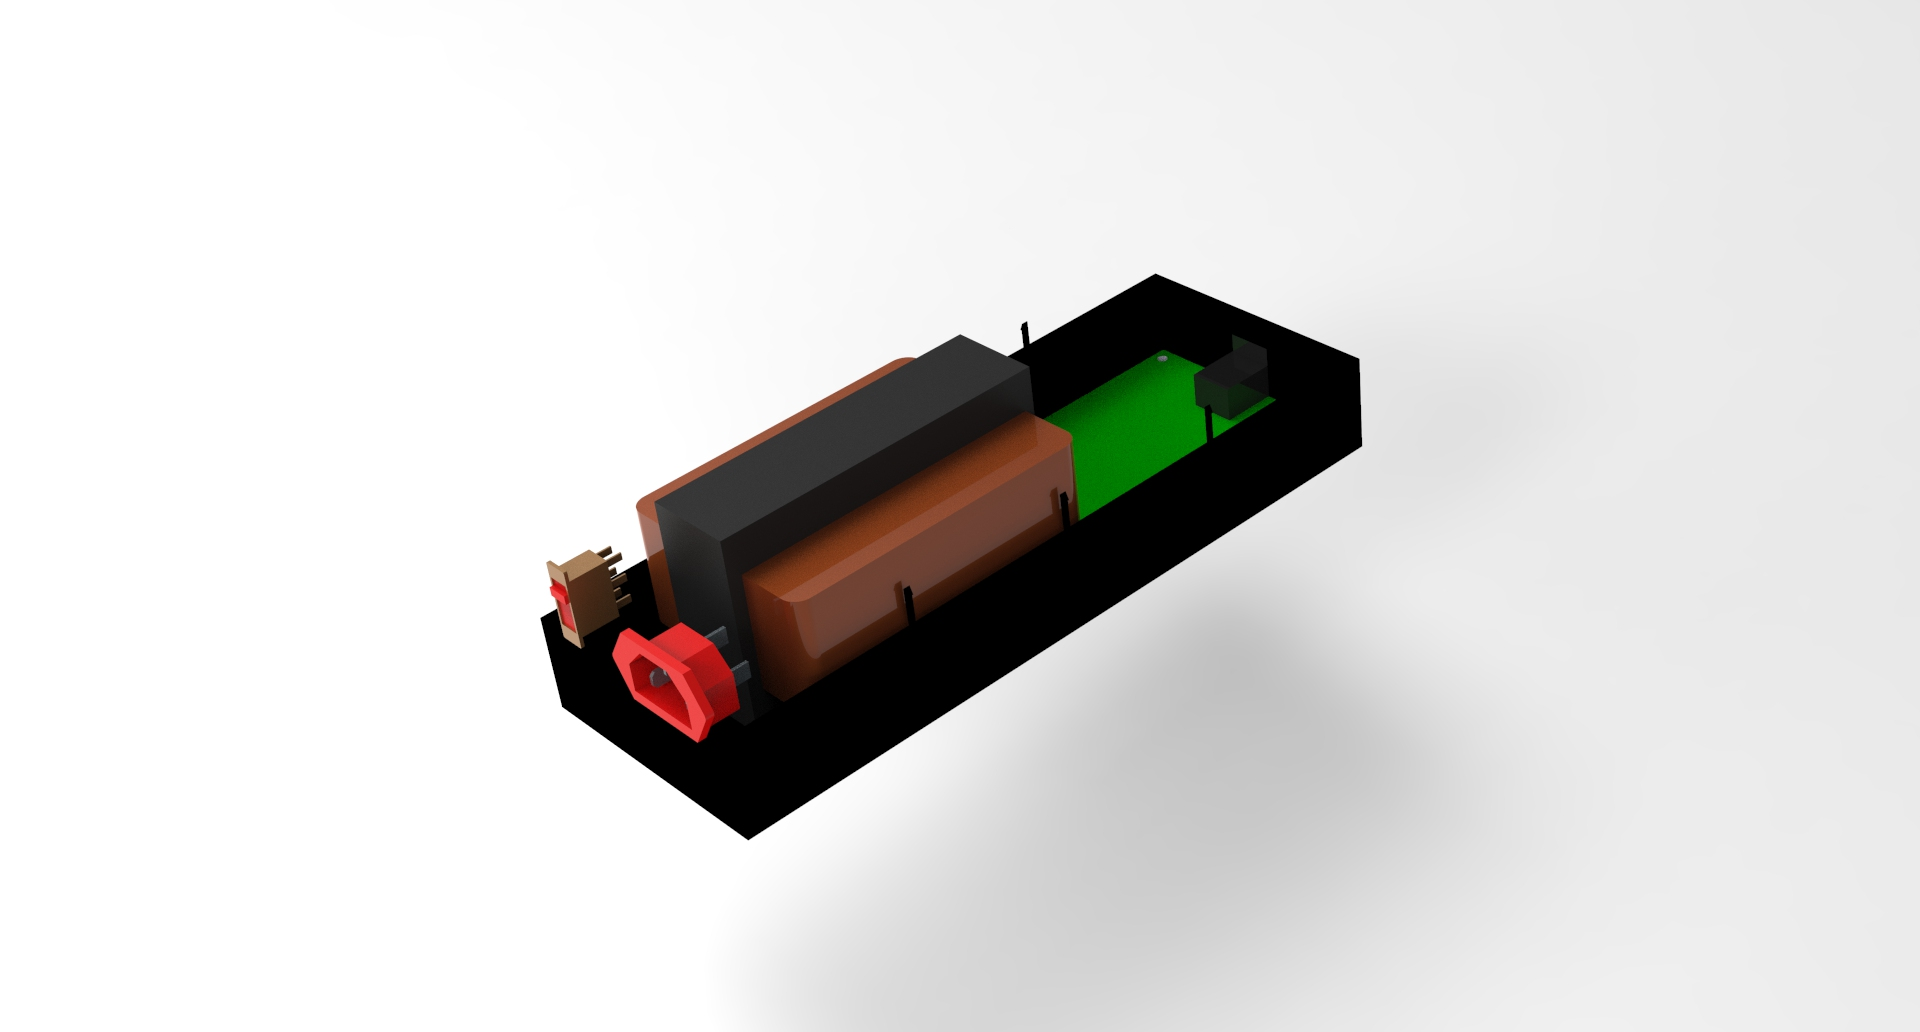
\includegraphics[width=0.7\textwidth]{figuras/cad/untitled.6.jpg}
\caption{Distribuição do Carregador}
\label{fig:carregador02}
\end{figure}

E por fim na figura \ref{fig:carregador03} é apresentado como ficou o projeto final do sistema com o carregador aberto onde é possível vê os encaixes de fechamento da case.

\begin{figure}[H]
\centering
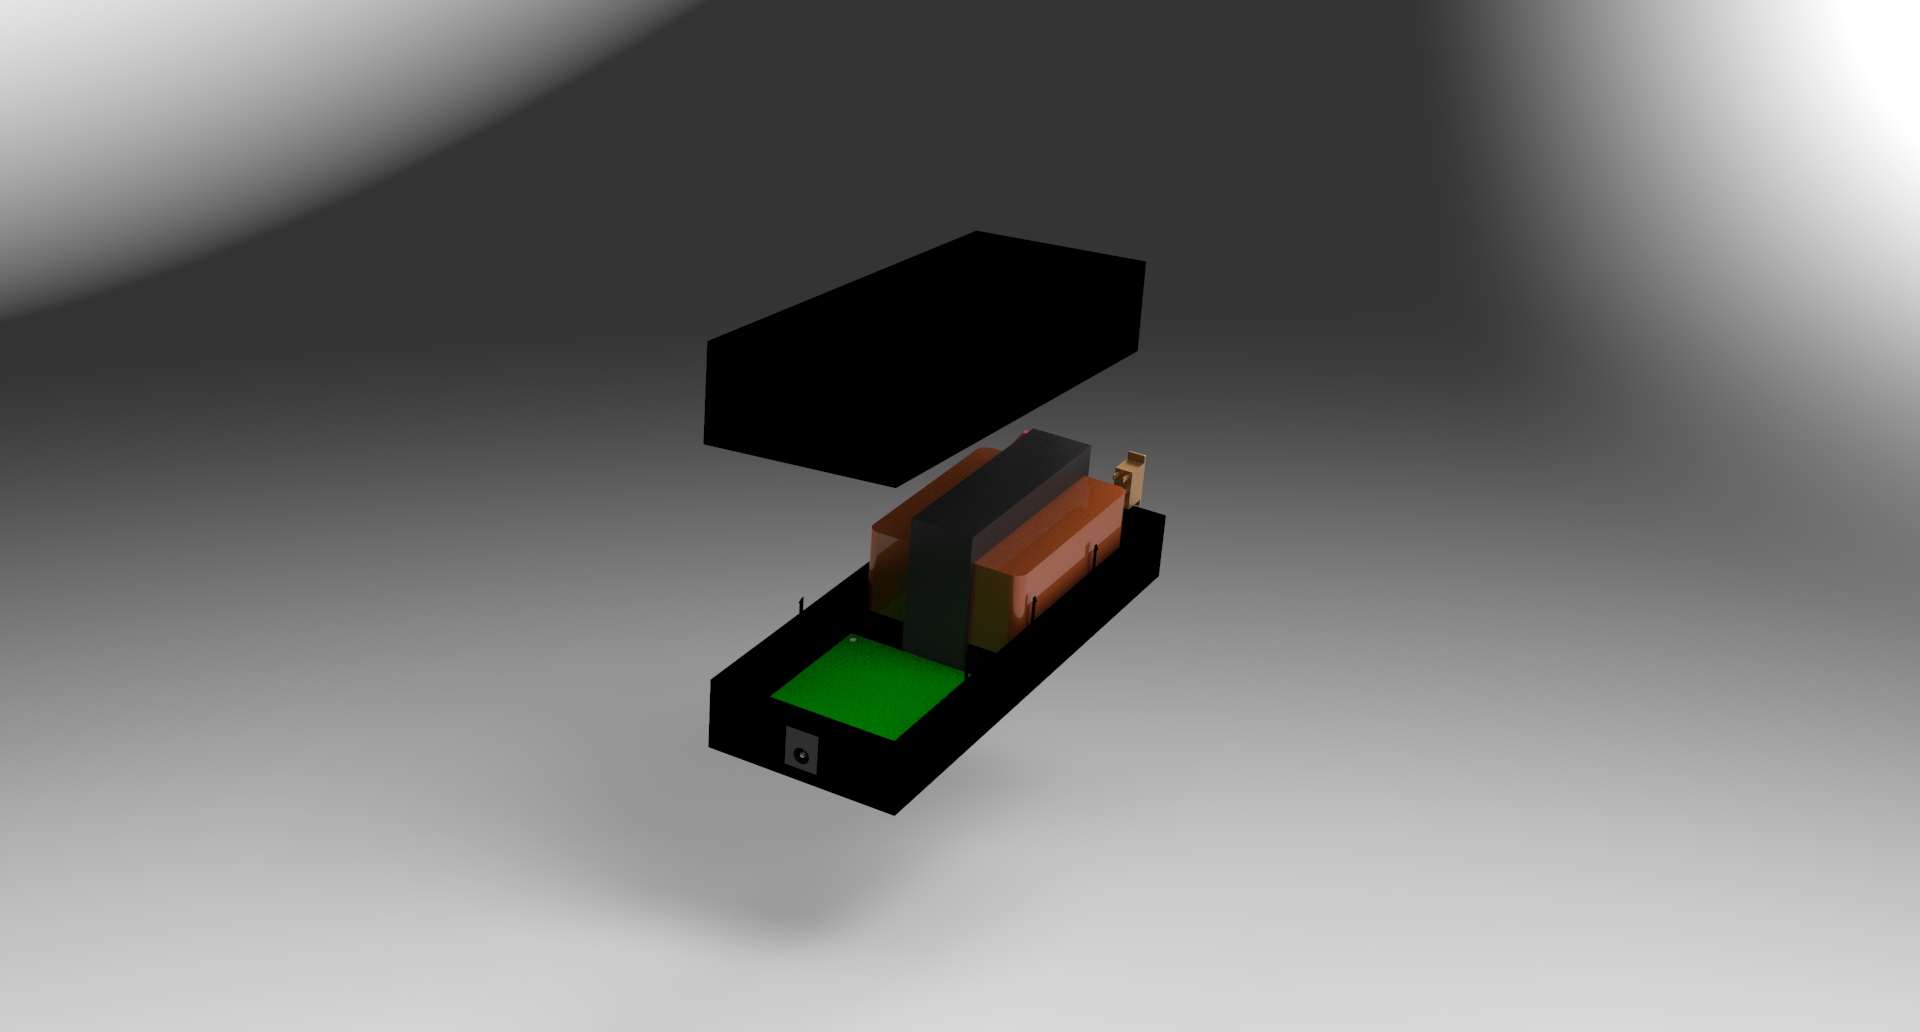
\includegraphics[width=0.9\textwidth]{figuras/cad/untitled.8.jpg}
\caption{Carregador Aberto}
\label{fig:carregador03}
\end{figure}

\subsection{Case base de lançamento}

\par Já a segunda case desenvolvida, foca na PCI desenvolvida pelo grupo de eletrônica na seção \ref{sec:base_de_lancamento}, onde um sistema eletrônico é instalado de forma a dá suporte ao sensor de carga utilizado pelo cliente. Dá mesma forma que na case do carregador, aqui são apresentadas nas figuras \ref{fig:base01}, \ref{fig:base02} e \ref{fig:base03}, imagens análogas ao do carregador para a case da base de lançamento.

\begin{figure}[H]
\centering
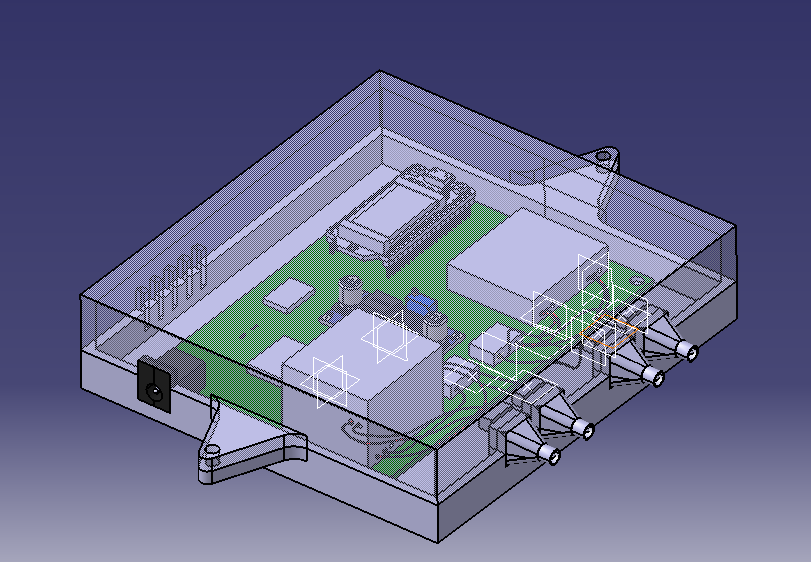
\includegraphics[width=0.7\textwidth]{figuras/cad/ISOCASELET.PNG}
\caption{Vista Isométrica da Case}
\label{fig:base01}
\end{figure}

\begin{figure}[H]
\centering
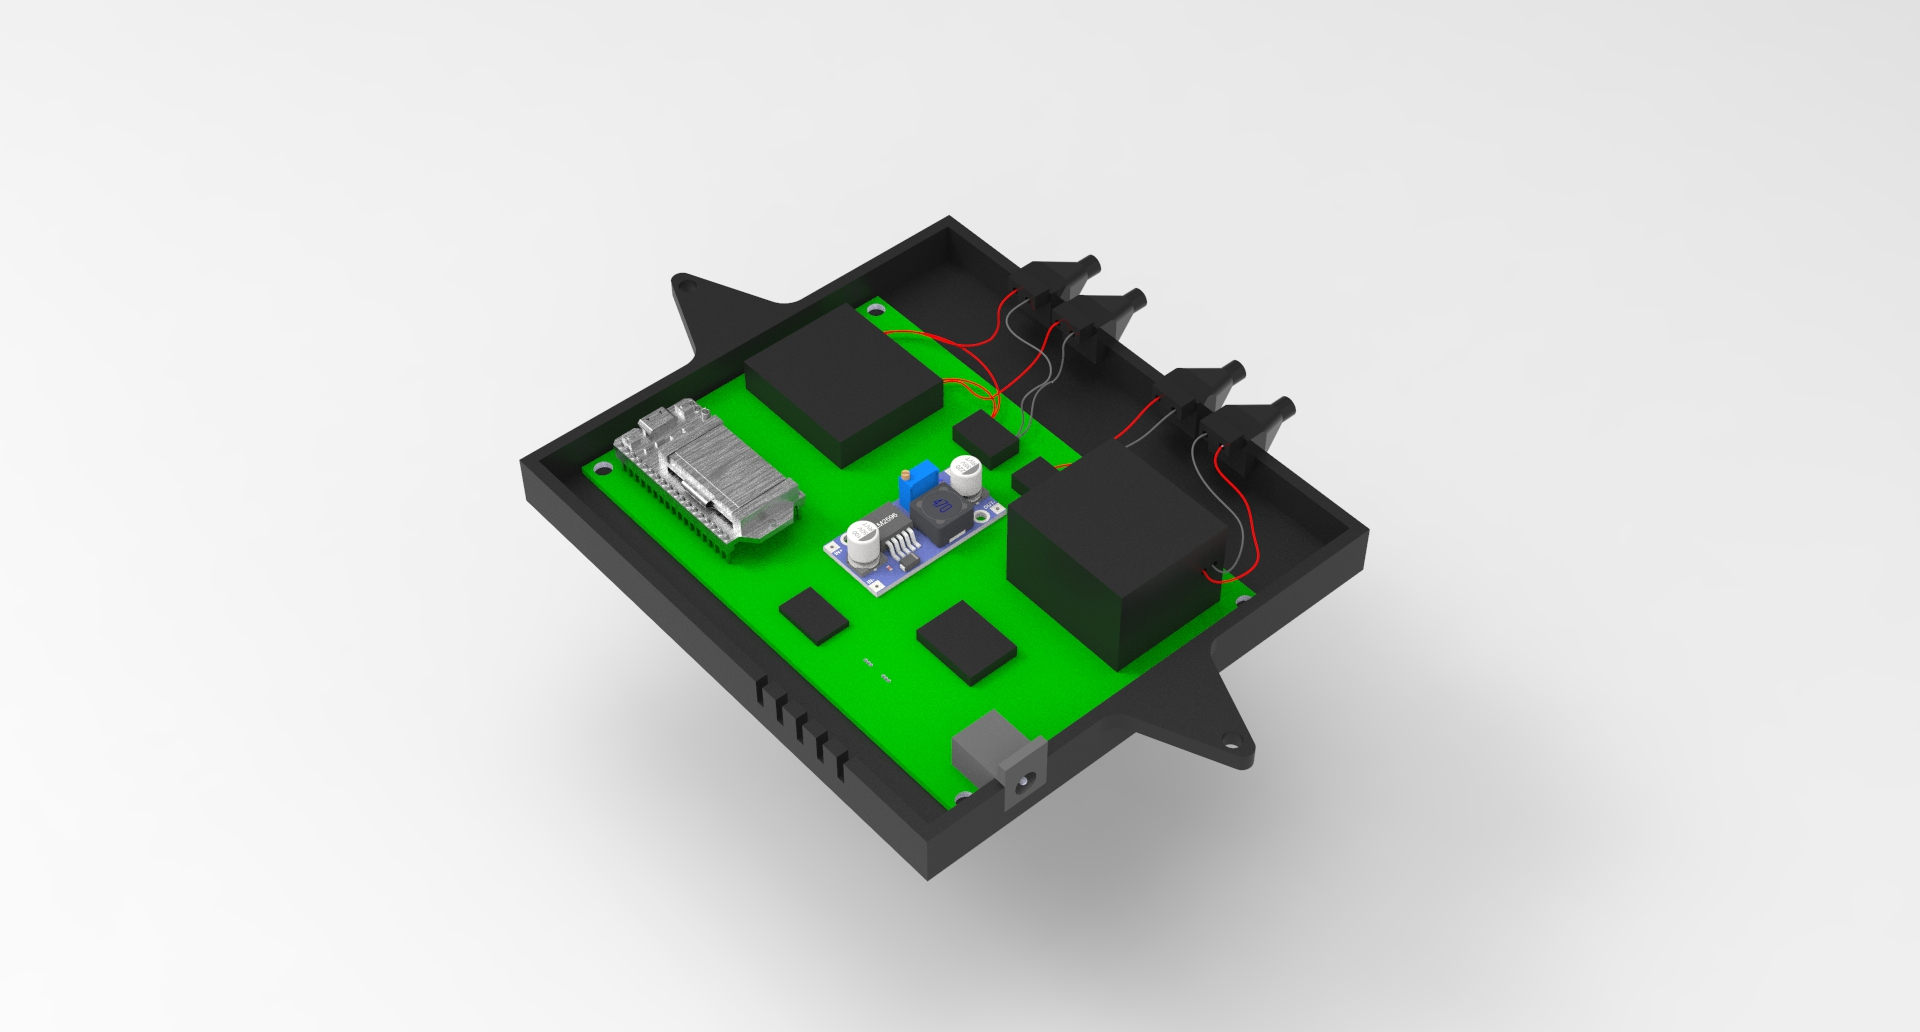
\includegraphics[width=0.7\textwidth]{figuras/cad/untitled.11.jpg}
\caption{Distribuição dentro da estrutura}
\label{fig:base02}
\end{figure}

\begin{figure}[H]
\centering
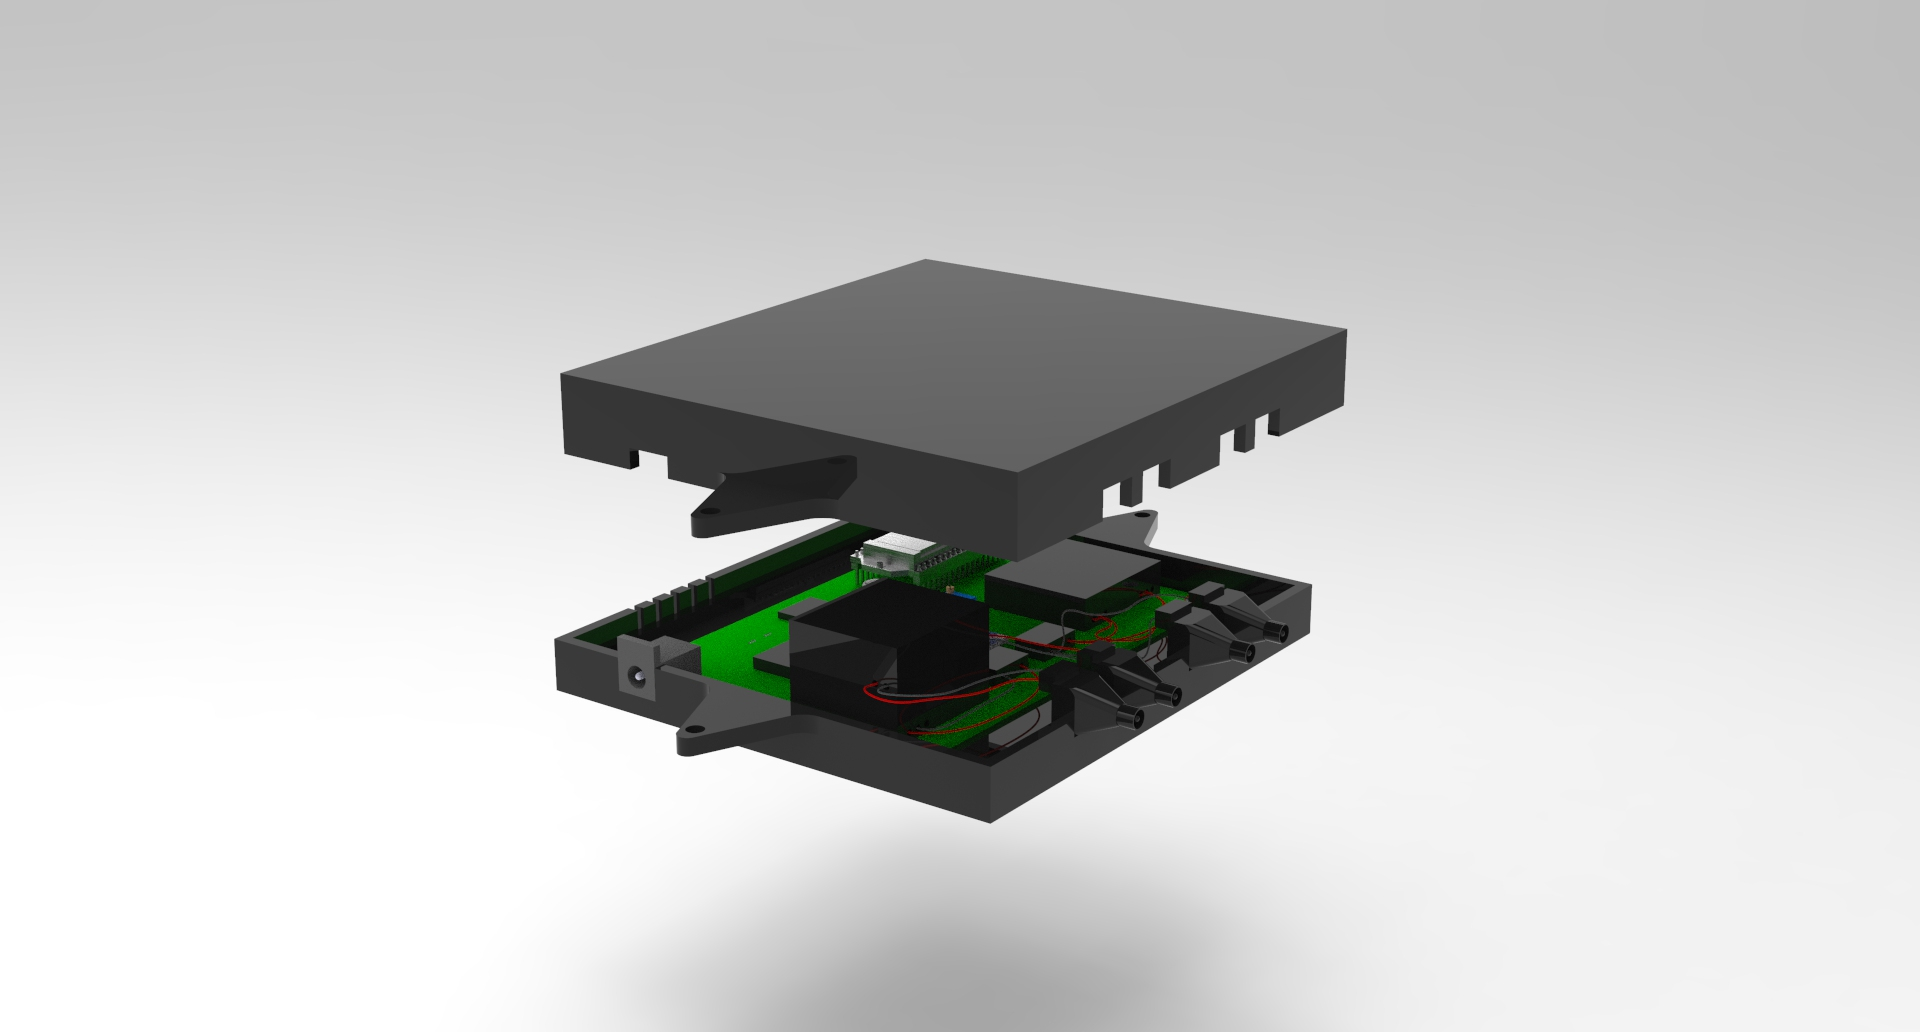
\includegraphics[width=0.9\textwidth]{figuras/cad/untitled.12.jpg}
\caption{Case aberta}
\label{fig:base03}
\end{figure}

\section{Simulações de Impacto}

\subsection{Razões para a simulação}

\par Inicialmente, era planejado pela equipe realizar uma simulação numérica, utilizando o \textit{software} Ansys, dos efeitos que esforços mecânicos possam gerar na estrutura das maletas, em particular a deformação que estas poderiam sofrer. No entanto, conforme orientado pelos professores durante a apresentação do Ponto de Controle 1, essas estruturas não vão receber carga durante seu funcionamento, exceto àquela exercida pelos pelo próprio peso das maletas. Logo, foi avaliado que esse tipo de simulação não traria resultados relevantes. Em lugar dessa simulação, foi sugerido então que se realizasse uma simulação numérica de impacto.

\par De fato, ao se pensar no uso recorrente de ambas as maletas, no qual ambas serão constantemente transportadas de um local ao outro, principalmente durante as preparações do lançamento, o esforço mecânico relevante que realmente tem mais chance de ocorrer é uma queda, a uma altura estimada de 1 metro, 1 metro e meio, caso esses sistemas estejam sendo usados de maneira correta (sendo transportado por uma pessoa na altura de suas mãos ou em repouso sobre uma mesa, no caso da maleta de controle). Desse modo, foi pensada uma situação hipotética em que ambas as maletas sofrem queda livre a uma altura de 1m em diversas posições de impacto. A simulação  tem por finalidade verificar os efeitos dessa queda.

\subsection{Preparação do modelo de simulação}

\par Para a realização dessa simulação, optou-se por desenvolver uma versão simplificada do CAD, baseado nas dimensões em cada uma das maletas e não considerando detalhes internos, como componentes eletrônicos, alças, dobradiças ou outras peças metálicas. Desse modo, foram desenvolvidos dois modelos de caixa oca, cada qual com as dimensões das maletas, com 15mm de espessura, de acordo com o tipo de chapa de MDF que fora escolhida para o projeto. A essas duas caixas, foi atribuído um material denominado "MDF", que fora adicionado à biblioteca do Ansys com base nas características mecânicas abaixo descritas.

\par Além desses modelos de caixa, foram desenvolvidos modelos de manta de SBR de 3 milímetros de espessura que envolvessem completamente ambas as caixas, de modo a realizar dois tipos de simulação: uma com as maletas sem revestimento e outra com a proteção do SBR. Da mesma forma que o MDF, foi criado um material intitulado "SBR" na biblioteca do Ansys, com base nas seguintes características  \cite{azomaterials} \cite{makeitfrom.com}:

    \begin{itemize}
        \item MDF
        \begin{itemize}
            \item Densidade: $750 kg/m^3$
            \item Módulo de Elasticidade: $4 GPa$
            \item Razão de Poisson: $0,25$
            \item Módulo de Cisalhamento: $1,6 GPa$
        \end{itemize}
        \item SBR
        \begin{itemize}
            \item Densidade: $940 Kg/m^3$
            \item Módulo de Elasticidade: $ 6MPa$
            \item Razão de Poisson: $0,48$
            \item Módulo de Cisalhamento: $2,03 MPa$
        \end{itemize}
    \end{itemize}

\par Por fim, foi elaborado um último modelo, representando o solo durante a queda, que consiste em um bloco 1000mm x 1000mm x 200mm, atribuindo-se o material concreto a partir da própria biblioteca de materiais do Ansys.

\par Para cada uma das duas maletas (com e sem revestimento), foram simuladas três situações de queda: queda direta, quando a maleta com a face inferior; queda lateral, quando a maleta cai com a face lateral voltada para baixo; e queda inclinada, quando a maleta cai "de quina", com inclinação de 45$^{\circ}$ nos eixos X e Z. Foram colhidos os resultados da tensão normal no sentido do eixo Y, da tensão de cisalhamento no plano XZ e da deformação.

\subsection{Detalhes da Malha}

Fora utilizada a ferramenta padrão do Ansys para geração da malha, cujos elementos tetraédricos tiveram o tamanho de 0,015m. Tentativas de  refinamento da malha, com aumento da discretização (i.e. redução do tamanho dos elementos), resultaram em erros no programa, resultantes da falta de capacidade computacional da máquina utilizada. Optou-se, então, por manter a malha inicialmente gerada.
\par Abaixo, encontra-se uma tabela com o número de elementos e o número de nós para cada caso de simulação (maleta de controle, maleta de alimentação, com e sem revestimento).

\begin{table}[H]
\centering
\begin{tabular}{|c|c|c|}
\hline
    Simulação & Elementos & Nós \\\hline

    Controle sem revestimento & 8361 & 13266 \\\hline
    Controle com revestimento & 10545 & 18010 \\\hline
    Alimentação sem revestimento & 7341 & 11984 \\\hline
    Alimentação com revestimento & 9555 & 17428 \\\hline
  
\end{tabular}
\label{table: numeroElementosNos}
\caption{Número de elementos e nós da simulação}
\end{table}

 Abaixo, vemos os detalhes da malha dos modelos de ambas as maletas nas Figuras \ref{malha_maleta} e \ref{malha_igniçãoRevestida}, a primeira sem revestimento, a segunda com o revestimento de SBR.
 
\begin{figure}[H]
	\centering
		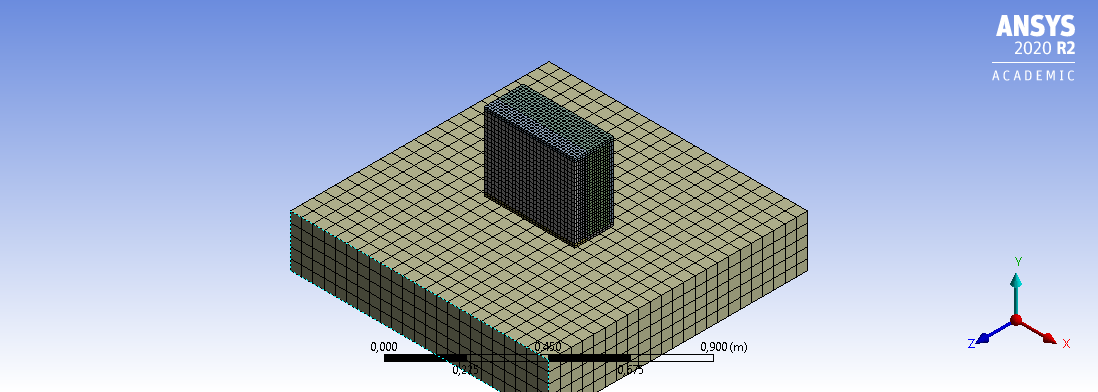
\includegraphics[width=1\textwidth]{figuras/estrutura_simulacaoImpacto/maletaMalha.png}
	\caption{Malha da maleta da estação de controle}
	\label{malha_maleta}
	\end{figure}

\begin{figure}[H]
	\centering
		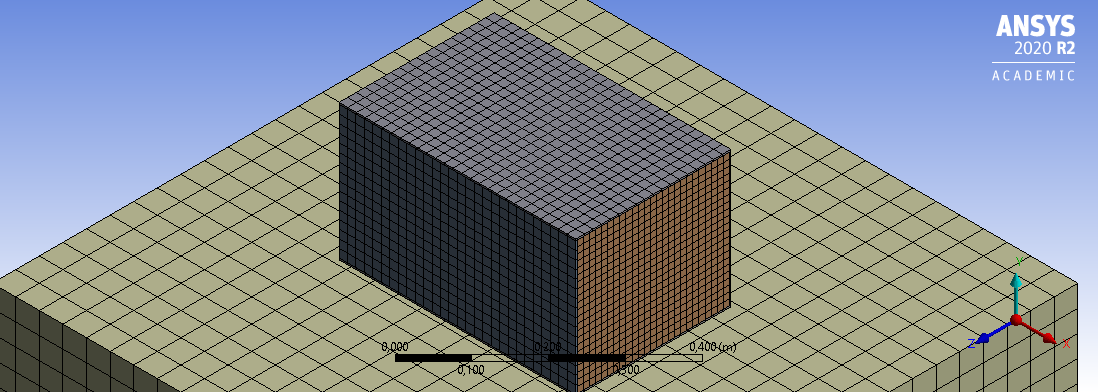
\includegraphics[width=1\textwidth]{figuras/estrutura_simulacaoImpacto/ignicaoRevestidaMalha.png}
	\caption{Malha da maleta do sistema de alimentação com revestimento}
	\label{malha_igniçãoRevestida}
	\end{figure}


\subsection{Condições iniciais}

\par Para a realização dessa simulação, foi considerada uma situação em que ambos os objetos atingem o solo a partir de uma condição inicial de repouso ($v_0 = 0$), em queda livre por uma altura $h = 1m$, sofrendo aceleração gravitacional constante de $g = 9,81 m/s^2$. Utilizando-se da equação de Torricelli \cite{hughd.young;rogera.freedman2008}:

\begin{equation}
    v^2 = v_0^2 + 2gh
\end{equation}
chegamos à velocidade a qual o objeto chega ao tocar o solo ($v = 4,4229 m/s$), velocidade esta que servirá de \textit{input} para a simulação.
\par Além disso, o corpo que representa o chão foi estabelecido como suporte fixo.



\subsubsection{Resultados e discussões}

As simulações geraram os seguintes resultados: tensão normal no eixo vertical (Y), tensão de cisalhamento no plano horizontal (XZ) e deformação. As imagens da distribuição das tensões, bem como a deformação, sobre o corpo do modelo em cada uma das simulações encontram-se no Apêndice \ref{simulacoes_impacto}. Abaixo, na Figura \ref{tabelaSimulacao}, encontram-se os valores máximos e mínimos das tensões em cada um dos casos definidos para análise numérica.


\begin{figure}[H]
	\centering

		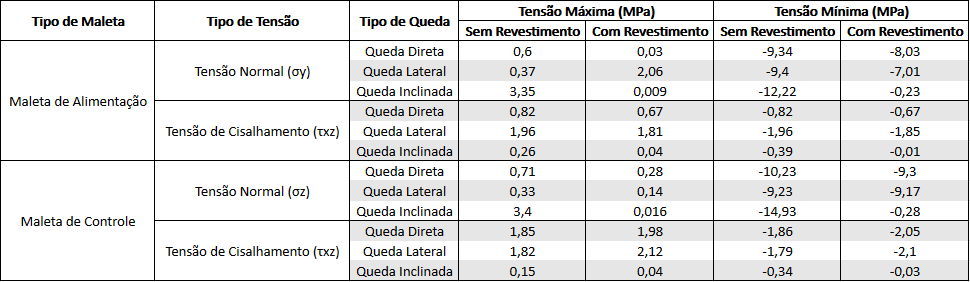
\includegraphics[width=1\textwidth]{figuras/estrutura_simulacaoImpacto/tabelaSimulacao.png}
	\caption{Tabela com as tensões máximas e mínimas de cada simulação}
	\label{tabelaSimulacao}
	\end{figure}

Os resultados corroboram a expectativa de que o revestimento reduziria a tensão máxima sofrida pelas maletas em todas as situações de queda simuladas. Vale destacar as quedas inclinadas, a redução chega a mais de $97\%$ do valor inicial de tensão. Isso é particularmente interessante, quando se trata de uma estrutura que comportará componentes eletrônicos delicados.
\par No entanto, vale ressaltar que, em se tratando de análise do material selecionado, os valores encontrados estão bem abaixo do módulo de ruptura do MDF conforme a Tabela \ref{tab:mdf}. De fato,é de se esperar que a estrutura resista a uma queda mínima como a simulada. Contanto que o usuário faça o uso recomendado das maletas, é bastante provável que esse tipo de impacto seja o mais recorrente, com consequências mínimas para a estrutura destas.
\par De todo modo, os resultados mostram que é válida a aplicação do revestimento de SBR, não somente pela redução da tensão sofrida pela estrutura das maletas, mas também por outras características da manta emborrachada, como a proteção contra intempéries ambientais e, em última análise, como material de sacrifício para o desgaste que as maletas venham sofrer. A escolha do uso do revestimento dependerá mais do quanto este pode afetar a construção das estruturas das maletas, como será visto adiante.
	
	
\section{Plano de construção}

\par Uma vez que os materiais e as dimensões das maletas foram definidos, foi elaborado o manual para a construção destas. O manual denominado Manual de montagem, apresenta o passo a passo para a construção de todos os elementos do projeto inclusive os das maletas. Este manual está presente no Apêndice \ref{Manual_de_montagem}. 

